%
%   Disserta��o: (colocar aqui nome pr�prio + apelido)
%		July 2018
%

% Sites / docs to check:
%
% MEEC:
% https://fenix.tecnico.ulisboa.pt/cursos/meec/documentos-e-regulamentos
% https://fenix.tecnico.ulisboa.pt/downloadFile/845043405460433/DMEEC201803.pdf
%
% IST:
% https://graduacao.tecnico.ulisboa.pt/alunos/dissertacao-de-mestrado/
% https://graduacao.tecnico.ulisboa.pt/files/sites/54/guia-de-preparacao-da-dissertacao-1516.pdf
% https://tecnico.ulisboa.pt/pt/recursos/documentos-importantes/


% --------------------------------------------------------- CONFIG:

\documentclass[a4paper,10pt]{book}
%\usepackage[latin1]{inputenc}   % incluir uma imagem postscript
%\usepackage[ansinew]{inputenc} 	% acentua��o autom�tica
\usepackage[portuguese,english]{babel}	% titles in last chosen language
\usepackage[utf8]{inputenc}
\usepackage[T1]{fontenc}
\usepackage{times}    					% poe letra bonita em PDF
\usepackage{indentfirst}		    % indenta o primeiro paragrafo de cada sec��o

%\usepackage[dvips]{graphicx}
\usepackage{graphicx}
\usepackage{float}
\graphicspath{{./}{./figs/}{../figs/}{../figs/sec2_event_camera/}{../figs/sec2_esim_dataset/}{../figs/sec2_camera_calibration/}{../figs/sec2_feature_detection/}{../figs/sec2_feature_tracking/}{../figs/sec2_ukf/}{../figs/sec2_imu/}} % share figs using ../figs/
\usepackage{subfigure}					% figuras paralelas ou seguidas com mesma legenda
\usepackage[outdir=./]{epstopdf}
\usepackage{color}

\usepackage{amssymb}
\usepackage{amsmath}
\usepackage{amsthm}          
%\usepackage[colorlinks=false, pdfstartview=FitV, linkcolor=blue, citecolor=blue, urlcolor=blue,breaklinks=true]{hyperref}
%\usepackage{subeqn}							% subnumerar equa��es

\usepackage{url}
%\usepackage{glossaries}
\usepackage[toc,style=long,acronym]{glossaries}
\usepackage{epigraph}
\setlength\epigraphwidth{8cm}
%\setlength\epigraphrule{0pt}
%\epigraph{``Begin at the beginning," the King said gravely, ``and go on till you
%come to the end: then stop."}{--- \textup{Lewis Carroll}, Alice in Wonderland}


%\usepackage{hyperref}   				% poe bookmarks no ficheiro pdf
%\PassOptionsToPackage{linktocpage}{hyperref}
\usepackage[linktocpage=true]{hyperref}

\usepackage{setspace}						% pacote de espa�amento
\usepackage{datetime}
\onehalfspacing									% espa�amento de 1,5 entre linhas
%\doublespacing			 

%\vspace{.5cm} 									% como por um espa�amento vertical

\textwidth 			=   16cm 				% largura do texto na folha
\textheight 		=   22cm 				%
\oddsidemargin 	= 	0cm 				% margens na folha
\evensidemargin =   0cm 				%
\marginparwidth =   0pt 				% margem de paragrafos
%\usepackage[top=25mm, bottom=25mm, left=25mm, right=25mm]{geometry}

\usepackage{fancyhdr} 					% cabe�alhos

\pagestyle{fancy}								% cabe�alhos do cap�tulo e sec��o em min�sculas
\renewcommand{\chaptermark}[1]{\markboth{#1}{}}
\renewcommand{\sectionmark}[1]{\markright{\thesection\ #1}}
\fancyhf{} % apagar as configura��es actuais
\fancyhead[LE,RO]{\bfseries\thepage}
\fancyhead[LO]{\bfseries\rightmark}
\fancyhead[RE]{\bfseries\leftmark}
\renewcommand{\headrulewidth}{0.5pt}
\renewcommand{\footrulewidth}{0pt}
\addtolength{\headheight}{4.5pt} % fazer espa�o para o risco
\fancypagestyle{plain}{%
	\fancyhead{} % Tirar cabe�alhos de p�gina vazias
	\renewcommand{\headrulewidth}{0pt} % e o risco
}


		%\includeonly{sec2_meth1}
		%\includeonly{sec3_meth2}
		%\includeonly{sec4_experiments}

		\includeonly{sec2_ukf}

% --------------------------------------------------------- MAIN:

\newglossaryentry{sae}
{
    name=SAE,
    description={Surface of Active Events is ...}
}

\newacronym{sae_ac}{SAE}{Surface of Active Events}
\newacronym{imu_ac}{IMU}{Inertial Measurement Unit}
\newacronym{ekf_ac}{EKF}{Extended Kalman Filter}
\newacronym{ukf_ac}{UKF}{Unscented Kalman Filter}


\makenoidxglossaries 

\begin{document}

%-------------------------------------------
% cover page
%-------------------------------------------

\thispagestyle{empty}

% -- Option 1/2 large letters:
\newcommand{\myfontA}{\LARGE} \newcommand{\myfontB}{\Large} \newcommand{\myfontC}{\large} 
% -- Option 2/2 large letters but not so large:
%\newcommand{\myfontA}{\Large} \newcommand{\myfontB}{\large} \newcommand{\myfontC}{\normalsize} 

\singlespace

% Logo -------------------------------------------

$ $ \vspace{-3cm}

\begin{minipage}[t]{5cm}
 %\includegraphics[width=\linewidth]{istlogo2.eps} % high res
 
\includegraphics[width=5cm]{istlogo3.eps} % IST logo 2013
\end{minipage}

%\begin{minipage}[t]{12.5cm}
%\centering
% \vspace*{-1.5cm}
% {{\myfontC \bf UNIVERSIDADE T�CNICA DE LISBOA}\\
%  {\myfontC \bf \vspace{0.2cm} INSTITUTO SUPERIOR T�CNICO}}
%\end{minipage}

\vspace*{-0.5cm} % \hspace*{-1.3cm}
\begin{center}
$ $ \\
\end{center}


%% Boneques ------------------------------------------------

%\begin{figure}[hbtp]
% \centerline{\includegraphics[height=4cm]{cover.eps}}
% \vspace{4mm}
%\end{figure}

% alternative to the Boneques:
\vfill

%% Title --------------------------------------------------
\onehalfspace
\begin{center}
  \myfontA
  {\bf Title of the Thesis}
\end{center}
%\vspace{7mm}
\singlespace


%% Author ---------------------------------------------------
\vfill

\begin{center}
  % place here the full name, i.e first, middle and last names
  {\myfontB \bf Full name} \\
  %(Licenciado)
\end{center}


%% Subject -------------------------------------------------
\vfill

%% Use the following if thesis title/contents is in Portuguese
%\onehalfspace
%\begin{center}
% {Disserta��o para a obten��o do Grau de Mestre em}\\
% $ $ \\
% {Engenharia Electrot�cnica e de Computadores}
%\end{center}
%\singlespace

%% Use the following if thesis title/contents is in English
\onehalfspace
\begin{center}
 {\myfontC Thesis to obtain the Master of Science Degree in}\\
 $ $ \\
 {\myfontB \bf Electrical and Computer Engineering}
\end{center}
\singlespace

%% Supervisor & juri ----------------------------------------------
\vfill

\onehalfspace

%% --- T�tulo da tese em Portugu�s => j�ri em Portugu�s
%\begin{center}
%{\myfontB \bf J�ri}
% $ $ \\
%\myfontC
% $ $      & {} \\
% { Presidente: Professor } \\
% { Orientador: Professor Jos� Ant�nio da Cruz Pinto Gaspar} \\
% { Co-orientador: Doutor } \\
% { Vogal: Professor } \\
%% { Vogal: } \\ % in case of more than one
%\end{center}

\begin{center}
{\myfontB \bf Supervisor} \\
%{\myfontB \bf Supervisors} \\
$ $ \\
\myfontC
 { Professor Jos� Ant�nio da Cruz Pinto Gaspar } \\
 %{ Professor  } \\
\end{center}

\vfill

%% --- English title => committee in English
\begin{center}
{\myfontB \bf Examination Committee} \\
$ $ \\
\myfontC
 { Chairperson: \emph{to be filled later} } \\
 { Supervisor: Professor Jos� Ant�nio da Cruz Pinto Gaspar} \\
 { Member: \emph{to be filled later} } \\
% {Member: } \\ % in case of more than one
\end{center}

\singlespace


%% Date ----------------------------------------------------
\vfill

\onehalfspace \centerline{\myfontB \bf \monthname \, \the\year} \singlespace

\pagebreak \thispagestyle{empty} $ $ \pagebreak
 \onehalfspacing 

\cleardoublepage \pagenumbering{roman}%


% NOTE1: An acknowledgments subsection is read by everyone, including people that knows nothing about the thesis AND no one revises it (even the supervisors).
% NOTE2: In order to include and acknowledgments subsection, please uncomment the next lines.
%
%\section*{Agradecimentos}
%\addcontentsline{toc}{section}{Agradecimentos}
%
%� com bastante satisfa��o que escrevo esta sec��o por finalmente ter vencido uma meta importante...


% -------------------------------------------------------------------------------

%\section*{Resumo}
%\addcontentsline{toc}{section}{Resumo}
%
%(Resumo em Portugu�s)
%
%
%\vspace{1cm}\noindent\textbf{Palavras chave:}
%C�mara pan tilt zoom, ...


\section*{Abstract}
\addcontentsline{toc}{section}{Abstract}

Although it is clear the intrinsic advantages of pan-tilt cameras with respect to fixed cameras, modern video surveillance systems are still based on networks of fixed cameras...


\vspace{1cm}\noindent\textbf{Keywords:}
Pan and Tilt Zoom Camera, ...


\tableofcontents % main index
\listoffigures
\listoftables

\glsaddall
\printnoidxglossary[type=\acronymtype,nonumberlist]

\printnoidxglossary[nonumberlist]

\cleardoublepage \pagenumbering{arabic}

\section{Introduction}

Many modern video surveillance systems encompass pan-tilt cameras due to the flexibility they provide in selecting the fields-of-view, as compared to using just fixed cameras. Although patent the great potential of using the pan-tilt cameras, one has to design pan and tilt controllers whose effectiveness directly impacts on the surveillance performance.
%
The work described within this dissertation ...


\subsection{Related Work} 

Related work, e.g. a simple to use camera calibration toolbox \cite{Bouguet}.

Related work, on another relevant subject ...


\subsection{Problem Formulation} 

% Identify one or two main difficulties in state of the art knowledge
% and briefly state how to approach those difficulties

Surveillance with pan-tilt cameras involves not only video processing but also controlling the pan and tilt angles. In this work ...


\subsection{Report Structure} 

Section 1 introduces the problem to approach in the thesis, in particular presents a short discussion on the state of the art on ... 
%
Section 2 presents ...
%
Section 3 describes ...
%
Section 4 provides an overview of the different experiments executed as well as the results attained.
%
Section 5 summarizes the work performed and highlights the main achievements in this work. Moreover, this section proposes further work to extend the activities described in this document.

The work described hereafter was partially published in (put ref here).

		%\section{Method 1}
\label{sec:meth1}

There is a large variety of segmentation algorithms...

		%\chapter{Method 2}
\label{sec:meth2}

One advantage of pan-tilt cameras with respect to fixed cameras is the capability of augmenting the surveyed area without adding extra complexity to the system...

		%\section{ Experiments }

This section describes the experiments performed to validate the methodologies presented and introduced in previous sections. Four experiments were performed addressing the ...


		%\section{ Conclusion and Future Work}

The work described in this thesis...

Two main technical constraints were originally identified in this work, (i) ... and (ii) ...

In particular we studied the ...

In future work we plan to extend the framework for multiple pan-tilt-camera scenarios, where questions like how to define regions of interest for a multiple pan-tilt-camera scene? or how to share information between the cameras? would arise.


\chapter{Background}
\label{sec:sec2}

\epigraph{We are like dwarfs on the shoulders of giants, so that we can see more than they, and things at a greater distance, not by virtue of any sharpness of sight on our part, or any physical distinction, but because we are carried high and raised up by their giant size}{--- \textup{Bernard De Chartres}}

\epigraph{``Ex nihilo nihil fit" (Nothing comes from nothing)}{--- \textup{Parmenides}}

Intro to section 2

 
\section{Event Cameras}
\label{sec:sec2_event}

Event cameras, also called neuromorphic cameras, silicon retina or dynamic vision sensor (DVS) are image sensors that respond to changes in brightness in the scene. Unlike conventional cameras, which capture full image frames at a fixed frequency (commonly 30Hz or 60Hz), producing redundant information and require a high bandwidth for transmission, each pixel in an event-based camera operate independently and asynchronously, reacting to changes of brightness in the scene, eliminating the transmission of redundant information, allowing for much higher temporal resolution (in the order of microseconds, as opposed to the milliseconds of conventional cameras).

Event cameras are inspired by the behaviour of the cells in the retina. Though oversimplified, retinal cells respond to changes in the environment (namely brightness), generating an electrical impulse. The transient response of each retinal cell is independent. Event cameras mimic this behaviour by asynchronously and independently responding to changes in brightness in the environment, generating ON/OFF events each time a predefined threshold in brightness is exceeded.

This architecture allows for interesting properties, such as microsecond temporal resolution, high dynamic range (above 120dB), which allows for scenes with both bright and dark zones, and does not suffer from under/overexposure, nor motion blur.

Events are triggered when the brightness in a certain pixel surpasses a certain threshold. In particular, discrete brightness steps are pre-defined, and whenever brightness detected crosses the threshold, an event is generated. Positive crossings generate ON events, and negative crossings generate OFF events. In effect, each pixel is constantly working as a comparator (with corresponding electronic to support this mode of working). Fig.\,\ref{fig:sec2_event_camera} shows the first-generation DVS sensor, with an array of 128x128 pixels (from \cite{lichtsteiner2008128}), where this idea of comparison and threshold is shown.

\begin{figure}[ht]
    \centering
    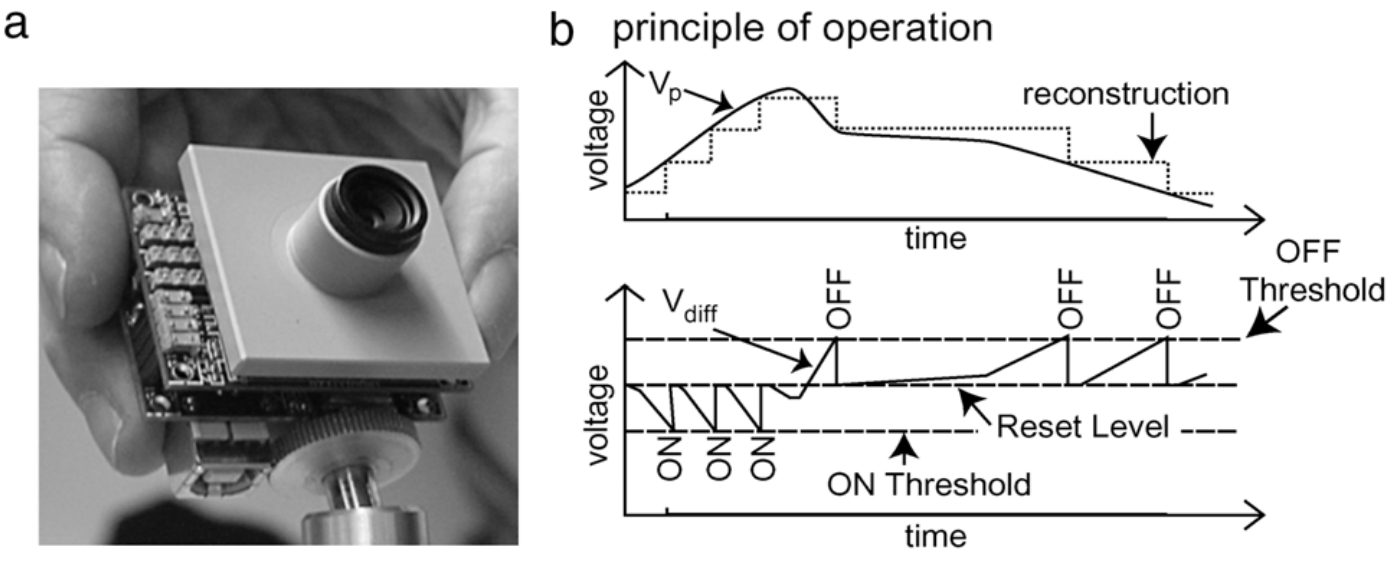
\includegraphics[width = 1\linewidth]{event_camera_principle.PNG}
    \caption[Event camera and operation principle]{First generation event camera (a) and corresponding principle of operation, showing the thresholds and the corresponding asynchronous generation of ON/OFF events, from \cite{clady2015asynchronous}}
    \label{fig:sec2_event_camera}
\end{figure}

Events are then defined as a four-component vector:

\begin{equation}
    \textbf{e} = \left(\left(x,y\right)^T,t,pol\right)^T = \left(\textbf{p},t,pol\right)^T
\end{equation}

The component $p=\left(x,y\right)^T$ refers to the spatial position of the event in the camera. The component $t$ refers to the timestamp of the event, and is of extreme importance due to the microsecond temporal resolution of the camera. Lastly, the parameter $pol$ refers to the polarity of the event (ON/OFF events).

With this event structure, it is common to represent events in a three-dimensional (space-time), representation, as shown in Fig.\,\ref{fig:sec2_space_time}, which shows the space-time evolution of events generated from a rotating black bar on a white background.

\begin{figure}[ht]
    \centering
    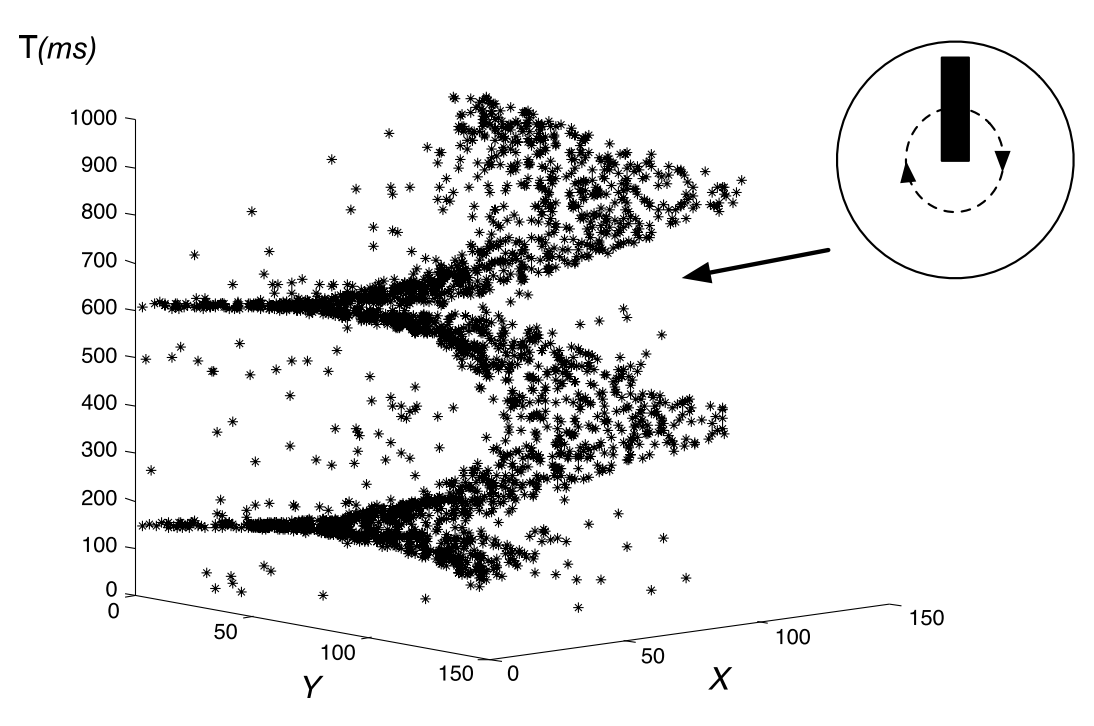
\includegraphics[width = 1\linewidth]{bar_rotating.PNG}
    \caption[Space-time representation of events generated from a rotating black bar]{Space-time representation of events generated from a rotating black bar, from \cite{clady2015asynchronous}}
    \label{fig:sec2_space_time}
\end{figure}

Conventional cameras and event cameras have fundamentally different modes of operation and output. As such, a comparison of the behaviour in the same scene, and an analysis of the output, is interesting. Fig.\,\ref{fig:sec2_standard_vs_event} shows the response of both a conventional camera and an event camera when presented with a disk rotating at a high speed, with a black dot. The fixed capture of the conventional camera is unable to keep up with the speed of the dot, and the images suffer from motion blur (not represented) and some discontinuity between frames. The event camera, however, due to its asynchronous event generation and temporal resolution, is able to continuously produce events relating to the movement of the dot.

\begin{figure}[ht]
    \centering
    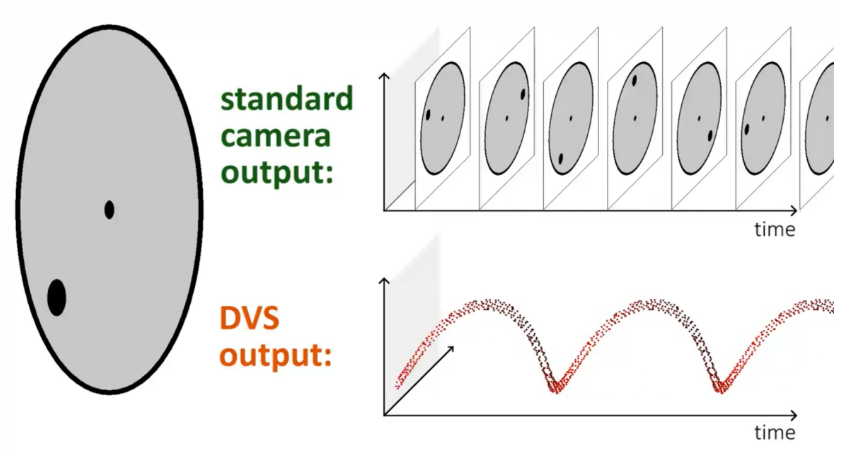
\includegraphics[width = 1\linewidth]{standard_vs_event.PNG}
    \caption[Comparison of the output of a standard camera and an event camera]{Comparison of the output of a standard camera (above), and an event camera (below), when recording a rotating disk with a black dot, from \cite{mueggler2017fast}}
    \label{fig:sec2_standard_vs_event}
\end{figure}

Advances in camera manufacturing have allowed for cameras that have both conventional camera pixel arrays, and event camera pixel arrays. This enables hybrid algorithms, which take advantage of the benefits of event cameras, with the extensive research on conventional cameras.  

\subsection{DVS240 and DAVIS240 event cameras}

A DVS240 event camera was used for this work. It is an event camera that is also capable of full frame greyscale recording (but not simultaneously with events, as only one can be active at each time; this mode was mainly intended for calibration purposes). The camera has a resolution of 240x180 pixels and comes with an adjustable length lens that changes the focal length (from 3.5mm to 12mm) and field of view (FOV) (from 64.6\,deg horizontal and 50.6\,deg vertical, to 20.9\,deg horizontal and 15.7\,deg vertical).

A more powerful camera, the DAVIS240, allows for the simultaneous recording of events and frames, and is the camera used in some of the datasets that were used, and is therefore worth mentioning. The rest of the specs are similar to the DVS240.

Lastly, ESim, an event camera simulator was also used in this work, and is explained further in Section\,\ref{sec:esim_dataset}.
\section{Camera Models and Calibration}
\label{sec:sec2_camera_model_calibration}

\subsection{Camera model}
\label{sec:sec2_camera_model}

The image obtained from a camera (either conventional or neuromorphic) results from the transformation of 3D points in the world to 2D points in the camera plane, and is constrained by the physical properties of the camera. Such properties include unwanted distortions relating to the lens' geometry, as well as unalignment between the lens and the camera sensor. 

The goal of the calibration is to estimate the intrinsic (parameters relating to the camera itself, such as focal length, optical centre, and skew coefficient, which are fixed), extrinsic (parameters external to the camera, specifically translations and rotations between the camera and the world) and distortion (relating to the lens) parameters of the camera. A calibrated camera is needed for computer vision algorithms, as the relation between points in the image and world frames needs to be known for distance estimation, 3D reconstruction, depth estimation, ...

Distortion can be modelled as tangential and radial distortion. Radial distortion is caused by the elliptical geometry of the lens, as light rays bend more near the edges than at the optical centre. Smaller lenses cause greater distortion. It is possible to have three types of radial distortion, namely negative, none, and positive, as shown in Fig.\,\ref{fig:sec2_radial_distortion}. Tangential distortion occurs when the lens is not perfectly parallel to the sensor, which happens during manufacture, as shown in Fig.\,\ref{fig:sec2_tangential_distortion}.

\begin{figure}[ht]
    \centering
    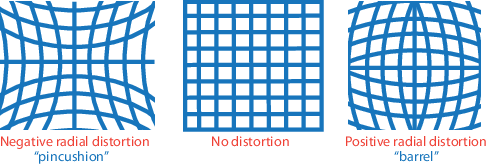
\includegraphics[width = 1\linewidth]{calibration_radial_distortion.png}
    \caption{Comparison of possible radial distortions}
    \label{fig:sec2_radial_distortion}
\end{figure}

\begin{figure}[ht]
    \centering
    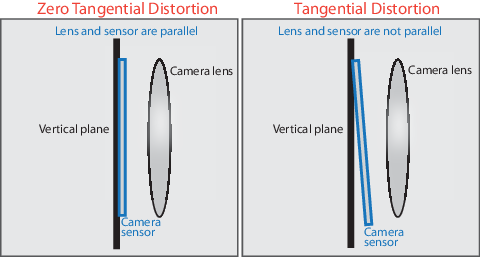
\includegraphics[width = 1\linewidth]{calibration_tangentialdistortion.png}
    \caption{Explanation for tangential distortion}
    \label{fig:sec2_tangential_distortion}
\end{figure}

Another important concept to take into account is that of camera model, which models the correspondence between points in the world and their position in image space. A common model used is the projective model (others can be used, such as perspective, affine, and orthographic models), in particular the pinhole model (Fig.\,\ref{fig:sec2_pinhole}). In this model, the mapping from world (3D) to camera (2D) is performed by tracing a ray of light from the world, through an infinitesimally small aperture (pinhole), and into the image plane. Important parameters in this model are the focal distance (distance from aperture to image plane), and image (or optical) centre (centre of the image plane), which are both intrinsic parameters. 

\begin{figure}[ht]
    \centering
    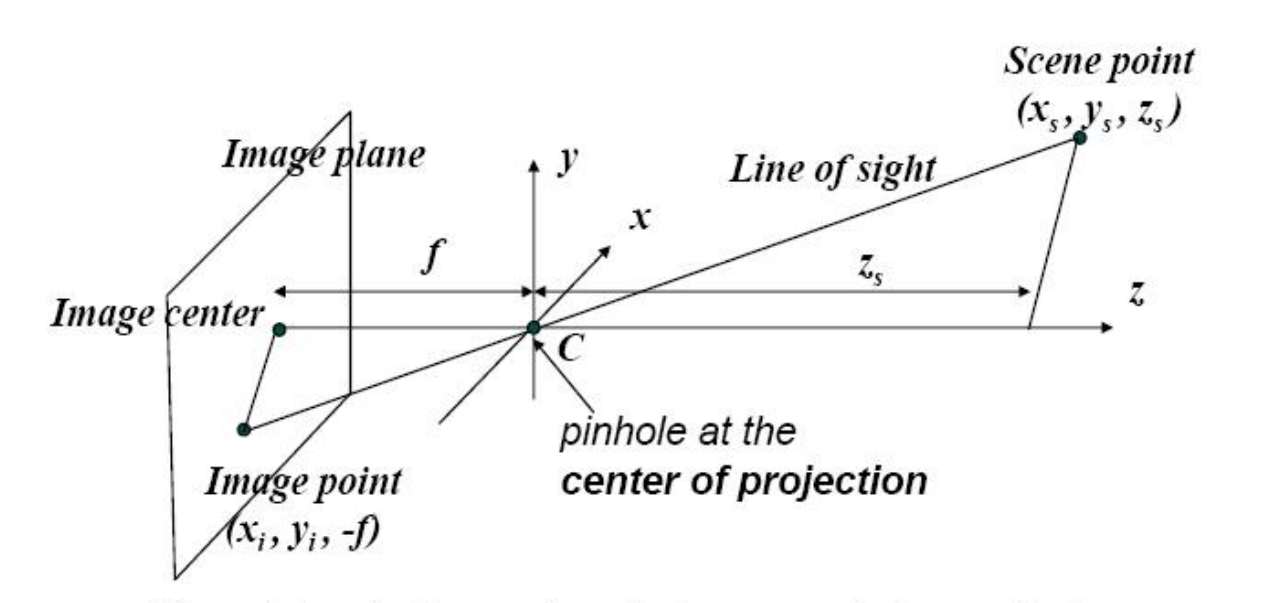
\includegraphics[width = 1\linewidth]{pinhole.png}
    \caption{Pinhole camera model}
    \label{fig:sec2_pinhole}
\end{figure}



From this model, we can derive the projective geometry, where the image plane is modelled in front of the optical centre, and the optical axis is orthogonal to the image plane. In this model, lines are projected to lines, collinear features remain collinear, and tangents and intersections are preserved, but parallel lines (in the world) eventually meet at a vanishing point, since angles are not preserved.

This geometry makes it clear that projection between world and image are given by the triangular similarity in Eq.\,\eqref{eq:sec2_projection}. 

\begin{equation}
    x=f\frac{X}{Z}, y=f\frac{Y}{Z}
    \label{eq:sec2_projection}
\end{equation}


\begin{figure}[ht]
    \centering
    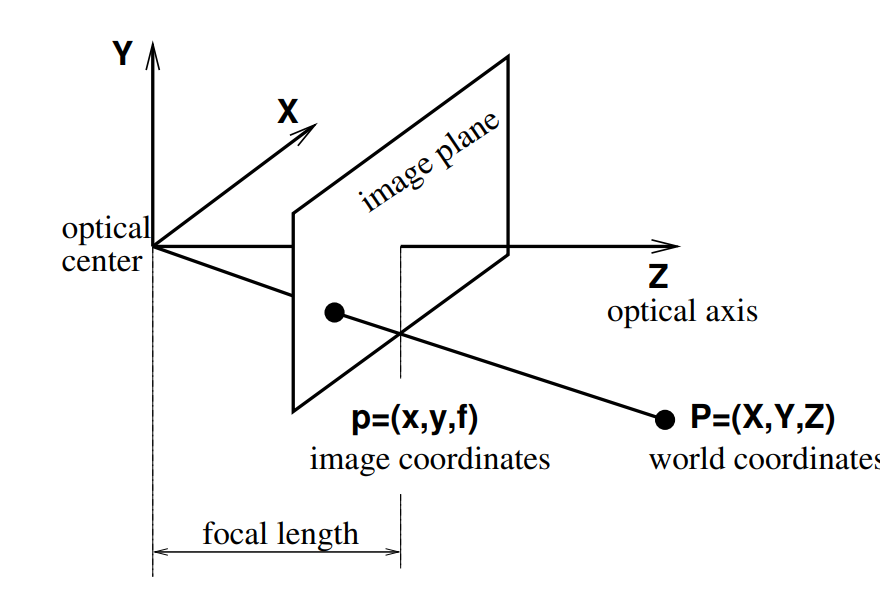
\includegraphics[width = 1\linewidth]{projective.png}
    \caption{Projective geometry}
    \label{fig:sec2_projective_geometry}
\end{figure}

The intrinsic parameters combine these properties, namely focal length ($f$), offset to the optical centre ($c_x$ and $c_y$), and skew ($s$, from non-orthogonality between optical axis and image plane), and constitute the intrinsic parameters matrix$K$, defined in Eq.\,\eqref{eq:sec2_instrinsic_matrix}. This matrix is also present in the projective matrix $P$, which relates the points in world space to their corresponding image plane position, shown in Eq.\,\eqref{eq:sec2_projective_matrix}, which is critical for computer vision.

\begin{equation}
    \label{eq:sec2_instrinsic_matrix}
    K=\begin{bmatrix}
        f_x & s & c_x\\
        0 & f_y & c_y\\
        0 & 0 & 1
    \end{bmatrix}
\end{equation}

\begin{equation}
    \label{eq:sec2_projective_matrix}
    \lambda \begin{bmatrix}
        x\\
        y\\
        1
    \end{bmatrix}=
    P
    \begin{bmatrix}
        X\\
        Y\\
        Z\\
        1
    \end{bmatrix}
    =
    \begin{bmatrix}
        K & 0
    \end{bmatrix}
    \begin{bmatrix}
        X\\
        Y\\
        Z\\
        1
    \end{bmatrix}
    =
    \begin{bmatrix}
        f_x & s & c_x & 0\\
        0 & f_y & c_y & 0\\
        0 & 0 & 1 & 0
    \end{bmatrix}
    \begin{bmatrix}
        X\\
        Y\\
        Z\\
        1
    \end{bmatrix}
\end{equation}

Assuming camera rotation and translation (extrinsic parameters, since image and world frames are not centred), the projective can be expanded to include rotation $R$ and translation $t$, and becoming completely generic, as shown in Eq.\,\eqref{eq:sec2_projective_matrix_rotation}. This is called the camera matrix.

\begin{equation}
    \label{eq:sec2_projective_matrix_rotation}
    x = K \begin{bmatrix}
        R & t
    \end{bmatrix}
    X
\end{equation}

\subsection{Camera calibration}
\label{sec:sec2_camera_calibration}

The process of finding the matrix K for a given camera is known as camera calibration. The calibration problem can be formulated as an optimization problem that matches 3D reference positions in the world, which can be either known (Direct Linear Transformation) or unknown), and the corresponding projections in the camera plane. We can assume centred image and world frames (ignore extrinsic parameters), and focus solely on intrinsic parameters, resulting in a total of 5 unknowns.

An example of calibration with known features is Direct Linear Transformation (DLT) \cite{tsai1987versatile}, in which we know the exact location of points in the 3D world and their corresponding image projection in the camera plane, and through linear equations that result from the mapping of multiple points through the camera matrix. Though this technique provides good results, a very careful setup is needed, as greater precision leads to better parameter estimation. This is not always possible, or very practical, which is why more flexible were proposed.

A popular technique is that of Zhang (\cite{zhang2000flexible}), which relies on a checkerboard planar pattern captured from at least two orientations. The high contrast of the checkerboard pattern allow for easy detection of edges and corners, as well as the plane of the checkerboard. A typical workflow consists of capturing a few images of the checkerboard under different orientations, by either moving the camera or the checkerboard, then detect feature points in the images and use a closed form solution to match 3D and 2D points, and obtain an estimation of the parameters. Afterwards, an energy optimization based on the maximum-likelihood criterion is used to fine-tune the parameters. 

\subsection{Event camera calibration}

Event cameras follow the same optical principles described in Section\,\ref{sec:sec2_camera_model}, meaning the same models are still valid, but suffer from the same distortion parameters that need to be quantified through calibration. However, due to the nature of event cameras, the techniques from Section\,\ref{sec:sec2_camera_model} cannot be applied directly. The static images of the checkerboard that are used in conventional camera calibration would just be blank images (because event cameras need movement or changes). Nevertheless, completely redesigning the last decades of computer vision calibration techniques is ill-advisable, and the technique for event cameras merely replaces the steps up until feature acquisition.

Event camera calibration is a two-stage procedure. First, a sharp image (such as the ones in Fig.\,\ref{fig:sec2_calibration_patterns}) is used, in order to focus the lenses (focus adjustment). With this procedure, the edges produced from moving the camera or the pattern should be sharp. 

\begin{figure}[ht]
	\centering
		\begin{tabular}{cc}
		   
\includegraphics[width=0.45\linewidth]{pattern.png} &
		   \hspace{1cm} 
\includegraphics[width=0.45\linewidth]{chessboardpattern.jpg} \\
		   (a) & (b)  \\
		\end{tabular}
	\caption{Example images used for focus adjustment}
	\label{fig:sec2_calibration_patterns}
\end{figure}




Afterwards, a blinking LED pattern is used (Fig.\,\ref{fig:sec2_blinking}). This pattern attempts to mimic the checkerboard of conventional calibration, and the LEDs act as the corners of the checkerboard. Usually, a grid of 5x5 LEDs, spaced 5\,cm between themselves, and blinking at a frequency of 500\,Hz is used. 


\begin{figure}[ht]
	\centering
		\begin{tabular}{cc}
		   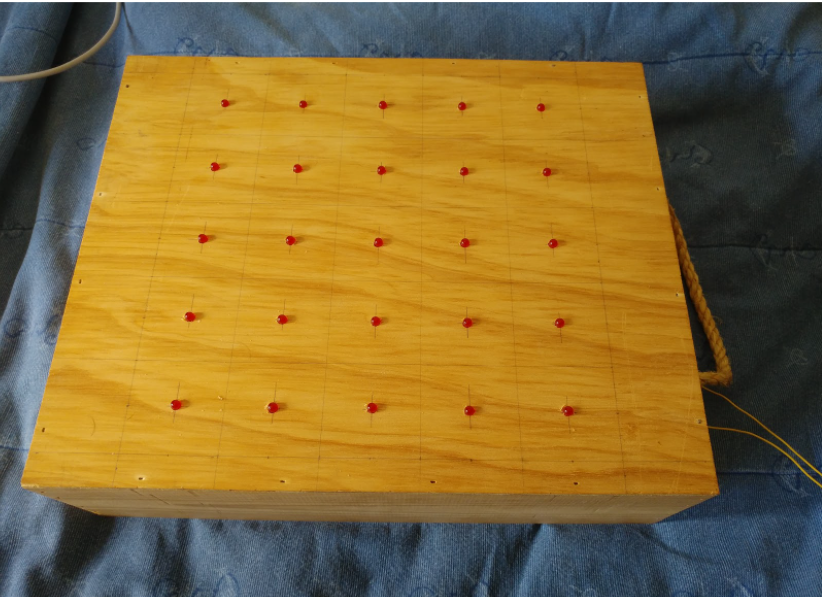
\includegraphics[width=0.45\linewidth]{box.png} &
		   \hspace{1cm} 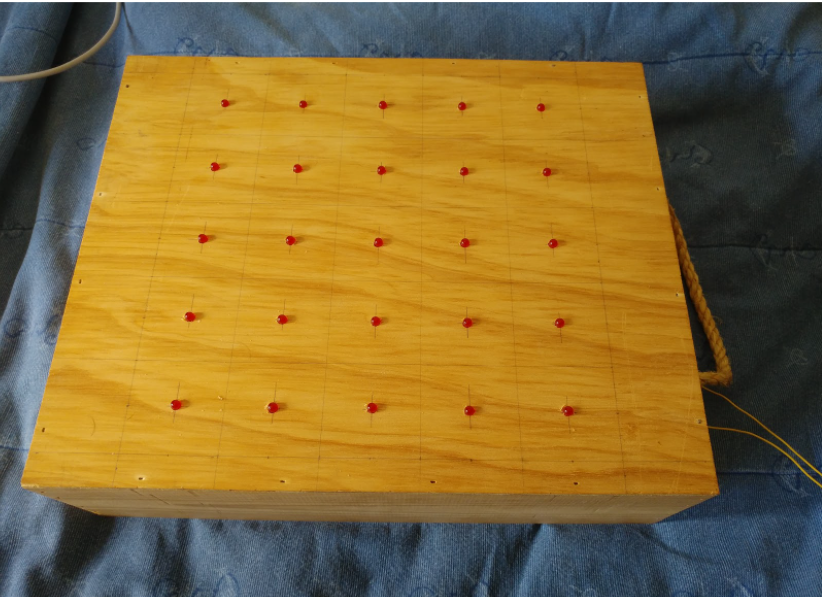
\includegraphics[width=0.45\linewidth]{box.png} \\
		   (a) & (b)  \\
		\end{tabular}
	\caption[Setup for event camera calibration]{(a) Schematic used for the connection of the LEDs, and (b) LED pattern in a rigid surface for calibration}
	\label{fig:sec2_blinking}
\end{figure}


Since the LEDs are blinking, the event camera is able to detect them and generate events, even with a still environment and camera. These events (from the blinking) are accumulated over a period of time in order to create a pseudo-frame, and blob detection is used to provide these feature to the pipeline of conventional camera calibration, which would use the corners as features. From here, the calibration pipeline is preserved.

Newer generation neuromorphic cameras combine both event and conventional camera (grayscale) acquisition. For these cameras, since the optical parameters are the same (same lens and same sensor), calibration can be performed using conventional techniques, or event camera specific techniques. The result should be the same (or similar).

% NOTA algumas imagens vieram daqui, mas nao sei mt bem como refernciar sites https://www.mathworks.com/help/vision/ug/camera-calibration.html
\section{IMU (Inertial Measurement Unit)}
\label{sec:sec2_imu}

The IMU is a sensor that reports the linear acceleration and the angular velocity of a body by means of accelerometers and gyroscopes (sometimes also the orientation by means of magnetometers, but the IMU used did not have this capacity and therefore it is not analysed).

Starting with the gyroscope, and considering a single axis, it provides a measurement $\tilde{\omega}$ that relates to the angular velocity of that axis, and is given by Eq.\,\eqref{eq:sec2_meas_model_gyr}, which corresponds to the true angular velocity $\omega$ corrupted by the sensor bias $\omega_b$ and the sensor noise $\eta_{\omega}$, which is modelled as additive, zero-mean Gaussian noise.

\begin{equation}
    \label{eq:sec2_meas_model_gyr}
    \begin{split}
        \tilde{\omega} = \omega + \omega_b + \eta_\omega\\
        \eta_{\omega} \propto \sim N\left( 0, \sigma_{gyro}^2 \right)
    \end{split}
\end{equation}

In order to have 3FOF we use 3 gyroscopes, one for each orthogonal axis, and we assume no crosstalk between them. The bias is temperature dependent and can vary over time, but is generally modelled as a constant, and may be specified in the manufacturer's datasheet, alongside the sensor variance $\sigma_{gyro}^2$.

In order to obtain orientation information from angular velocity, we can integrate the angular velocity, as per the motion equations and corresponding Taylor expansion \eqref{eq:sec2_taylor_gyro}.

\begin{equation}
    \label{eq:sec2_taylor_gyro}
    \begin{split}
        \omega(t) = \frac{\partial}{\partial t} \theta(t) \\
        \theta(t+\delta t) \approx \theta(t) + \frac{\partial}{\partial t} \theta(t) \delta t + \epsilon\\
        \epsilon \propto O(\delta t^2)
    \end{split}
\end{equation}

A perfect measurement would produce a perfect estimation of orientation (apart from a constant offset). However, noise makes this more complicated, as shown in Fig.\,\ref{fig:sec2_gyr_noise_int}. Gaussian noise makes the orientation estimation fluctuate along the correct value, which may be acceptable in some situations. However, the bias poses a more complicated problem, as we are constantly integrating a wrong value, even when there is no movement.

\begin{figure}[H]
	\centering
		\begin{tabular}{cc}
		   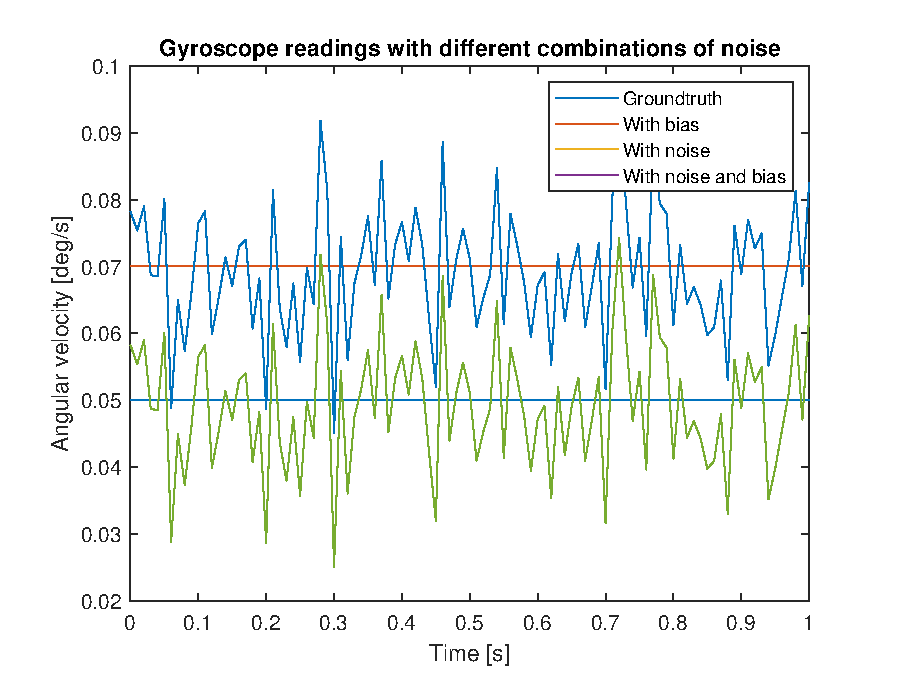
\includegraphics[width=0.45\linewidth]{gyr.eps} &
		   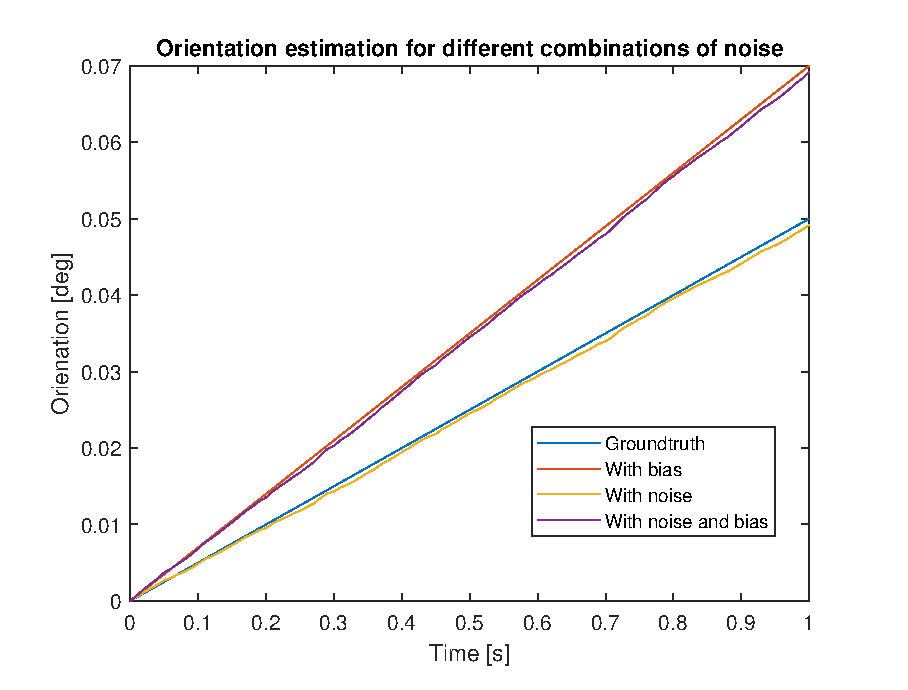
\includegraphics[width=0.45\linewidth]{or.eps} \\
		   (a) & (b) \\
		\end{tabular}
	\caption[Effect of noise on IMU]{(a) Effect of the various types of noise on the reading of the sensor and its impact on the estimation of the orientation (b)}   
    \label{fig:sec2_gyr_noise_int}
\end{figure}

Continuing with the accelerometers, a similar reasoning can be applied. We have a measurement $\tilde{a}$ given by Eq.\,\eqref{eq:sec2_meas_model_acc}, dependent on the true value $a$, sensor bias $a_b$ and noise $\eta_a$.

\begin{equation}
    \label{eq:sec2_meas_model_acc}
    \begin{split}
        \tilde{a} = a + a_b + \eta_a \\
        \eta_a \propto \sim N\left( 0, \sigma_{acc}^2 \right)
    \end{split}
\end{equation}

Again, a sensor for each axis is used, and no crosstalk is assumed. In order to obtain position information from angular velocity, we can integrate the acceleration twice (once for velocity and twice for position), as per the motion equations and corresponding Taylor expansion \eqref{eq:sec2_taylor_acc}.

\begin{equation}
    \label{eq:sec2_taylor_acc}
    \begin{split}
        v(t) = \frac{\partial}{\partial t} x(t) \\
        a(t) = \frac{\partial}{\partial t} v(t) = \frac{\partial^2}{\partial t^2} x(t)\\
        x(t+\delta t) \approx x(t) + \frac{\partial}{\partial t} x(t) \delta t + \frac{1 \partial^2}{2 \partial t^2} x(t) \delta t^2+ \epsilon\\
        \epsilon \propto O(\delta t^3)
    \end{split}
\end{equation}

Similarly, a perfect measurement would produce a perfect estimation of position (apart from a constant offset), but noise and bias render this task difficult. An extra step needs to be taken into account, which is the force of gravity, that needs to be subtracted from the affected axis (or axes, when no single axis is pointing straight down (or up)).

IMUs are very useful in the sense that they provide high speed information regarding both position and orientation (through angular veloxity and linear acceleration). However, the noisy measurements, coupled with the random walk associated with the bias, can lead to very incorrect estimations, especially when the system is standing still, and the noise overpowers the correct measurement itself.

\subsection{IMU calibration}

Just like the camera needs calibration, so do other sensors, in particular the IMU. In order to minimize the effect of noise and bias in the estimation, it is important to characterise these parameters. Ideally, they are supplied by the manufacturer in the datasheet. Oftentimes, however, they are not, and it is necessary to experimentally determine them.

We used the Kalibr framework \footnote{https://github.com/ethz-asl/kalibr} to characterise these parameters. \cite{board1998ieee} introduces the technique used by Kalibr, which consists of recording sensor measurement while standing still for a large amount of time (at least 4 hours), and then creating a plot with the log-log Allan deviation, as shown in Fig.\,\ref{fig:sec2_allan}. Two curves are then fitted to the plot, one with slope $-1/2$, and a second with slope $1/2$.

$\sigma_{gyro}$ and $\sigma_{acc}$ are taken directly at $\tau = 1$s, as we assume the noise power in most inertial sensors is dominated by noise at this frequency (point 1 in the plot). $\omega_b$ and $a_b$ corresponds to the value at which the line with slope $1/2$ crosses $\tau = 3$s (point 2 in the plot).

\begin{figure}[ht]
    \centering
    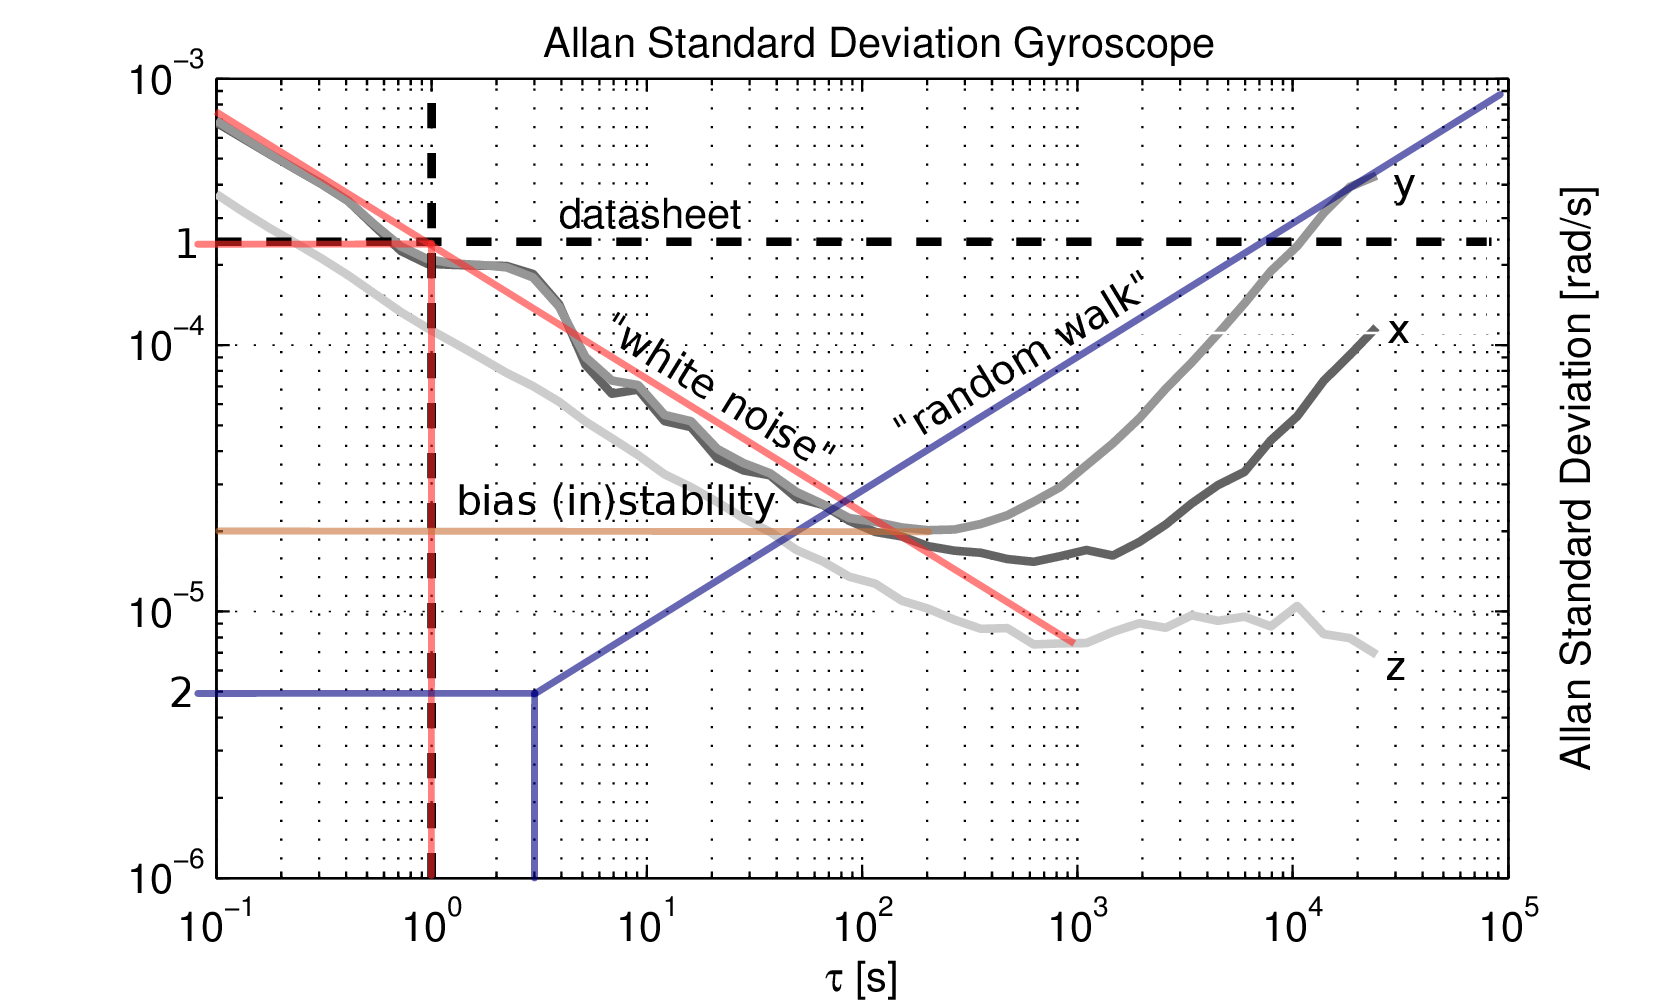
\includegraphics[width = 1\linewidth]{allan.png}
    \caption[Calibration of IMU through Allan standard deviation fitting]{Allan standard deviation of a gyroscope, showing the fitted lines, and noise characterisation, from the Kalibr wiki}
    \label{fig:sec2_allan}
\end{figure}

\section{ESIM Simulator and Event Camera Datasets}
\label{sec:esim_dataset}

Research on event cameras and event-based computer vision is still in its early stages. One of these reasons is tied to the hardware itself, since event cameras are expensive, not widely available, and are mostly prototypes, with low resolution (no more than 346x260 in the case of a state-of-the-art DAVIS346) and therefore not ready for commercial applications. Another such reason is the need for data and datasets, which are also scarce for the time being.
    
To tackle these problems, a number of simulators have been developed, of which ESIM (\cite{rebecq2018esim}) is an example, developed by Depts. Informatics and Neuroinformatics at ETH Zurich, in a similar spirit to the  conventional cameras simulator available. ESIM is an open-source ROS package.

\subsection{Simulators and ESIM}

Most event camera simulators continuously render images, and consecutive frames are compared. Events are then generated from big enough differences between frames.

A common problem with this technique is the choice of framerate, as a naïve approach would have the engine render at 1000 frames per second, in order to match the microsecond temporal resolution of event cameras. However, this is not ideal, as many frames are redundant, and therefore performance is affected. An ideal approach would only generate frames that are guaranteed to generate events, but at the same time should have a temporal resolution comparable to event cameras. ESIM uses a tightly coupled system between the simulator and the rendering engine, allowing for a better simulation, by using an adaptive sampling rate based on the dynamics of the scene.

Fig.\,\ref{fig:sec2_comparison_sampling} shows the advantage of an adaptive sampling approach as opposed to a uniform sampling approach. In the latter, rapid changes in the environment are sometimes overlooked.

\begin{figure}[ht]
    \centering
    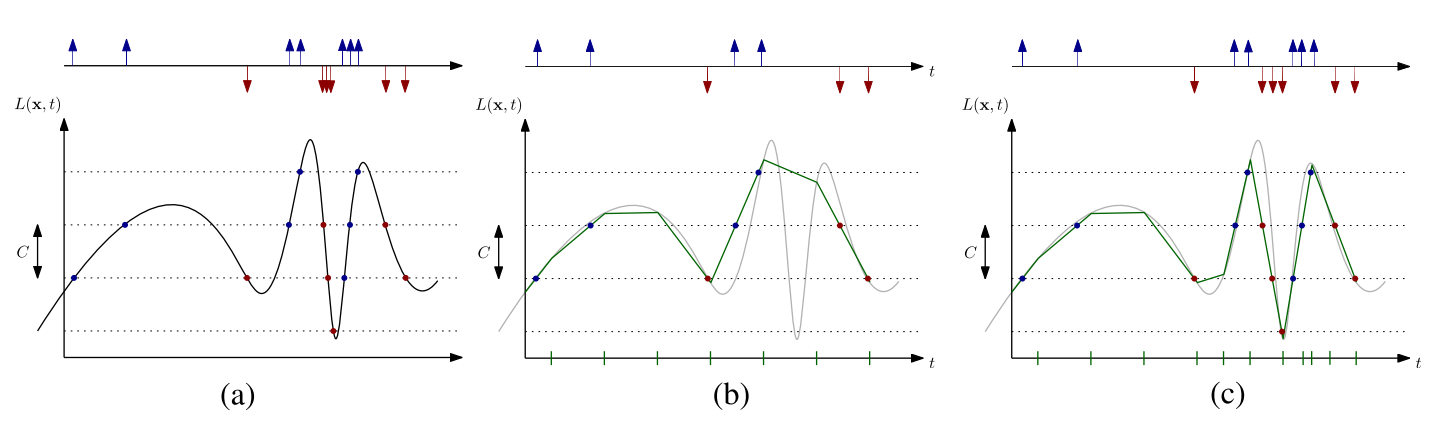
\includegraphics[width = 1\linewidth]{comparison_sampling.PNG}
    \caption[Comparison of sampling approaches for the simulator]{Comparison of a uniform sampling approach (b) and an adaptive sampling approach (c) when recreating the reference response shown in (a), from \cite{rebecq2018esim}}
    \label{fig:sec2_comparison_sampling}
\end{figure}

 This adaptive sampling is possible due to a communication between the simulator itself, and the rendering engine being used. It relies on the knowledge of the trajectory of the virtual camera to estimate the motion on the scene, which is used to guess changes due to brightness, pixel displacement, noise and non-idealities, to adapt the sampling rate and the event generation. Fig.\,\ref{fig:sec2_esim_architecture} shows the ESIM architecture.

 \begin{figure}[ht]
    \centering
    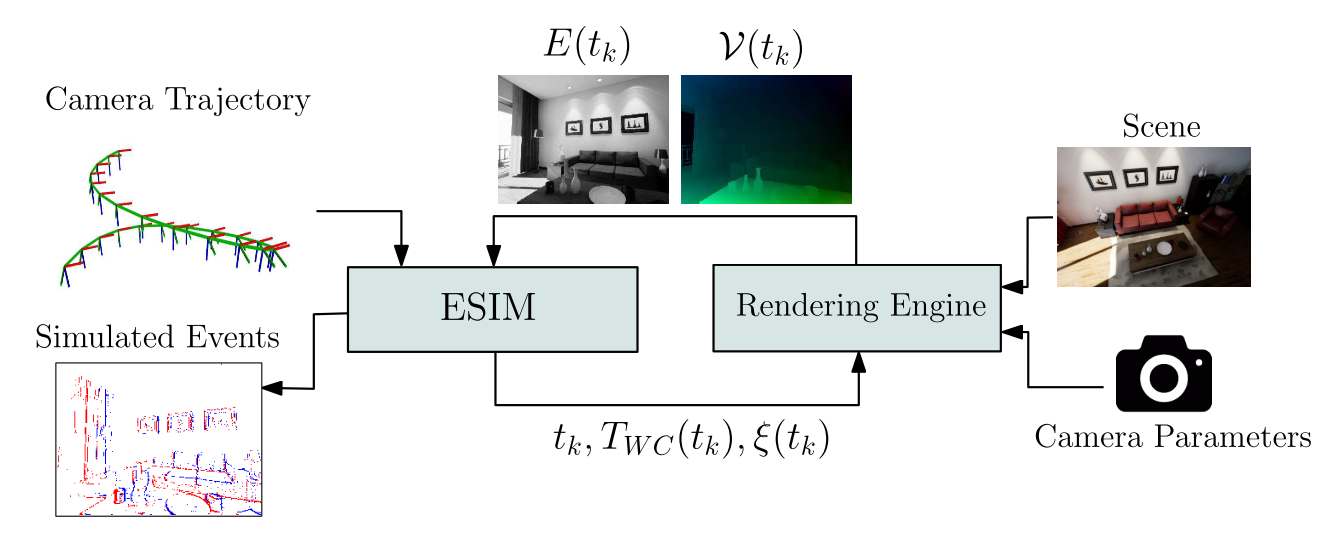
\includegraphics[width = 1\linewidth]{esim_architecture.PNG}
    \caption[ESIM architecture]{Architecture of ESIM, showing the tight coupling between the simulator and rendering engine, sharing the information of time $t_k$, camera pose $T_{WC}(t_k)$ and camera twist $\xi(t_k)$, generating irradiance map $E(t_k)$ and motion field map $\nu (t_k)$, from \cite{rebecq2018esim}}
    \label{fig:sec2_esim_architecture}
\end{figure}

ESIM allows the use of multiple rendering engines and modes, such as as an OpenGL integration, as well as a photorealistic rendering using Unreal Engine. The simulation of stereo cameras, and panoramic cameras is also possible. Furthermore, it is possible to “convert” videos to events, though the results are not as good, due to the fixed sampling rate of the videos, and unusage of the rendering engine.

The generation of events is as previously described. This simulator also allows for the generation of images, in effect replicating the more advanced DAVIS event cameras. For the generation of frames, a simple capture of the render from the viewpoint of the camera is performed, at specific intervals, corresponding to the framerate of the camera being generated. It is also possible to simulate exposure time, producing images that are subject to motion blur (useful for a "fairer" comparison in high-speed motions).

The trajectory performed by the virtual camera is crucial for generating the sensor readings, in particular the IMU measurements (which include both accelerometer and gyroscope readings), as well as groundtruth trajectory values (for posterior validation of methods). An explanation of the type of information provided by IMUs is included in Section\,\ref{sec:sec2_imu}.

The simulator can generate a random trajectory, by defining a random set of points, and can also receive a trajectory predefined in a file. In both cases, the points being supplied are only indicative, and internally the simulator fits a spline to the trajectory. This concept is shown in Fig.\,\ref{fig:sec2_traj_sup_ob}, and is crucial to generate a smooth trajectory that can be continuously differentiable (notice the jagged trajectory supplied and the smooth trajectory received, shown in Fig.\,\ref{fig:sec2_traj_sup_ob}). 

\begin{figure}[ht]
	\centering
		\begin{tabular}{cc}
		   \includegraphics[width=0.45\linewidth]{supplied.eps} &
		   \hspace{1cm} \includegraphics[width=0.45\linewidth]{obtained.eps} \\
		   (a) & (b)  \\
		\end{tabular}
	\caption[Trajectory obtained through simulator and provided trajectory]{Comparison of the trajectory that was supplied to the simulator (a) vs. the trajectory that was performed by the simulator (b), and provided in the trajectory groundtruth. The trajectory corresponds to a movement in a single axis, back and forth}
	\label{fig:sec2_traj_sup_ob}
\end{figure}


The importance of the smooth trajectory is that it can be directly related to the sensor readings. Taking the accelerometer, for example, it measures the linear acceleration of the camera in space. Well, the acceleration of a body can be given as the second derivative of movement (the first derivative being velocity). Likewise, velocity and position can be obtained (apart from a constant) by integrating the acceleration. 

As a result of a the smooth trajectory from the spline, which is continuously differentiable, we can obtain the accelerometer reading for that axis by deriving the trajectory twice, as shown in Fig.\,\ref{fig:sec2_comp_imu}, which compares the accelerometer reading obtained by differentiating the trajectory twice, and the reading that was in fact generated by the simulator. It is possible to observe they coincide, apart from a slight noise and bias that the simulator generates in order to generate more realistic data.

\begin{figure}[ht]
	\centering
		\begin{tabular}{cc}
		   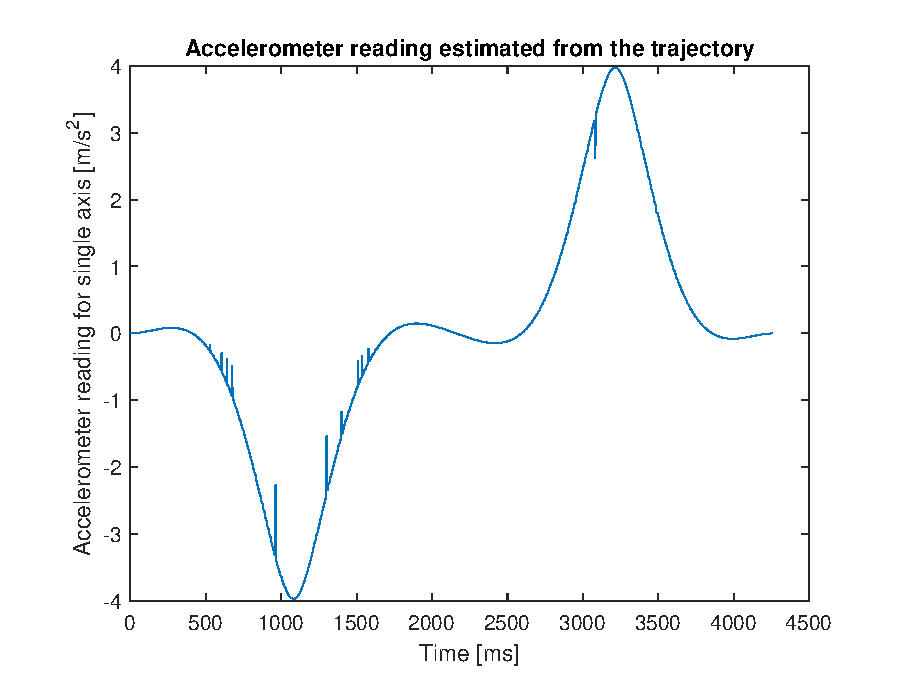
\includegraphics[width=0.45\linewidth]{acc_est.eps} &
		   \hspace{1cm} 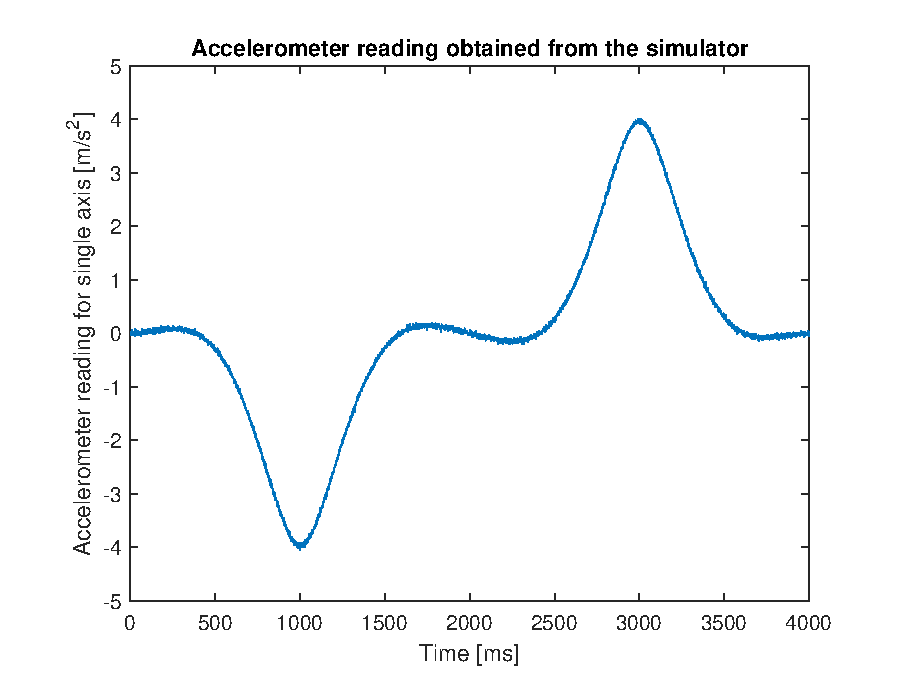
\includegraphics[width=0.45\linewidth]{acc_sim.eps} \\
		   (a) & (b)  \\
		\end{tabular}
	\caption[Comparison of sensor readings provided by simulator and the second derivative of the trajectory]{Comparison of the accelerometer reading obtained by differentiating the trajectory twice (a) vs. accelerometer reading that was obtained from the simulator (b). Notice the simulator adds some noise to simulate a real sensor. The spikes in (a) result from the discrete approximation of the derivative, but are not relevant for the relevance of the point being made and the comparison.}
	\label{fig:sec2_comp_imu}
\end{figure}

Likewise, for the other sensor readings (namely gyroscope), a similar approach is used, but instead taking the first derivative of the rotation along the trajectory.


\subsection{Datasets}

Datasets, like simulators, provide an interesting way to test algorithms without the need for a camera, compare results with other algorithms, and have a ground truth with which to benchmark.

The Depts. Informatics and Neuroinformatics at ETH Zurich provides a set of event camera datasets, recorded with a DAVIS 240C (an event camera with both events and full frames), along with IMU measurements and ground truth  (position and orientation) from a motion-capture system. Some of these datasets were used to test the algorithms developed.

Also, artificial datasets were generated through ESim, also to validate the algorithms developed with an accurate groundtruth.

%The datasets I have used are shapes_6dof.bag, which contains footage from a DAVIS240 of a collection of geometric shapes on a wall, and boxes_6dof.bag, which contains footage from a DAVIS240 of multiple boxes, with a complex texture.


\section{Feature detection}
\label{sec:sec2_feature_detection}

In the context of computer vision and image processing, image features are distinctive landmarks in the images, preferably unsusceptible to point-of-view, scale, and the aperture problem. Features are important as they provide information on the image, which can be used for recognition, matching, reconstruction, and tracking, among many other applications. Many types of features can be considered, such as edges, corners, blobs, ridges, and shapes.

The process of identifying features in an image is called feature detection, and multiple detectors have been described in the literature, dependent on the features of interest, such as Canny and Sobel detectors (for edges), Hough transform (for shapes), Laplacian operator (for blobs), and Harris detector (for corners).

For event-based cameras, new types of features, as well of detectors, are being proposed, as classical techniques are not easily transferable in most cases, or result in a non-negligible performance decrease, due to conversion overhead from asynchronous events to frames. However, corners seem to prove as interesting features to use, as not only can they be used to match features between the event stream and full frame images, allowing for sensor fusion, native event algorithms are available, which leverage the potential of events, namely speed and event independence.

\subsection{Classic corner detection}
\label{sec:sec2_classic_corner_detection}

The typical example for a classic corner detector is the Harris Corner Detector (\cite{harris1988combined}). It works using the following steps:

\begin{itemize}
    \item Compute the x-wise $I_x(x,y)$ and y-wise $I_y(x,y)$ partial image derivatives
    \item Compute the second-order derivatives $I_x^2(x,y)$  and $I_y^2(x,y)$, and cross-derivatives $I_x I_y(x,y)$
    \item Compute the second-moment matrix $M(x,y)$
    \item Compute the Harris score
    \item Detect local extrema whose Harris score is greater than the set threshold
\end{itemize}

The partial derivatives are computed by applying a Sobel derivative kernel (usually 3x3 or 5x5 kernels) to the whole image, producing the x-wise $I_x (x,y)$ and y-wise $I_y (x,y)$ partial image derivatives. From these derivatives, we can define the vector $\nabla I(x,y) = (I_x (x,y),I_y (x,y))^T$ and the second-moment matrix for each pixel ($M(x,y)$), defined as $M(x,y)= \sum_{(x,y)\in patch}^{}g(x,y)\nabla I(x,y)\nabla I^T(x,y)$, where $g(x,y)$ is a Gaussian weighting function centred around $(x,y)$, which controls the “sharpness” of the edge.

Then, we can compute the Harris score as defined in Eq.\,\eqref{eq:sec2_harris_score}.

\begin{equation}
    \label{eq:sec2_harris_score}
    H(x,y)=\lambda_1\lambda_2-k\times \left( \lambda_1 + \lambda_2 \right)^2 = det(M) - k\times trace (M)^2
\end{equation}

Where $k$ is an empirical value, $k \in \left[ 0.04; 0.06 \right ]$.

Finally, if $H(x,y)\geq H_0$, we consider the pixel as a corner. This will produce corner blobs. In order to select a single pixel to represent the corner, we select the local extrema (the pixel with the highest Harris score).

Another option to evaluate the presence of corners is to analyse the eigenvalues of M. If both eigenvalues are low, no interesting features are detected. If one is low, but the other is high, we are in the presence of and edge. Lastly, if both eigenvalues are high, the pixel is likely a corner. As such, one interpretation of the Harris detector is that corners are identified by finding the intersection of edges.

With this in mind, an alternative for the corner analysis, is to check the value of the lowest eigenvalue of $M (\lambda_{min})$, through the approximation Eq.\,\eqref{eq:sec2_min_eig}.

\begin{equation}
    \label{eq:sec2_min_eig}
    \lambda_{min} \approx \frac{\lambda_1\lambda_2}{\lambda_1+\lambda_2}=\frac{det(M)}{trace(M)}
\end{equation}

And then this value is used as a corner criterion.

\subsection{Event-based corner detection}
\label{sec:sec2_event_corner}

Due to the nature of events, gradient operators are not possible (at least directly applied to the event stream), since there is no image on which to apply them, and multiple techniques have been proposed, of which three will be presented.

\subsubsection{Space-time detection}
\label{sec:sec2_space_time}

This method relies on the space-time properties of events, and creates a 3D representation, containing the spatial position of an event $(x,y)$, as well as the time it was received. In this representation, edges moving with uniform linear speed create planes (stack of lines at different instants), and corner movement creates lines (stack of points at different instants).

As such, this technique tracks moving edges by fitting planes in this 3D representation, implicitly estimating the speed of the moving edge (optical flow). Each new event is matched to the previously estimated planes, and the estimates are updated, as shown in Fig.\,\ref{fig:sec2_plane_distance}. 

\begin{figure}[ht]
    \centering
    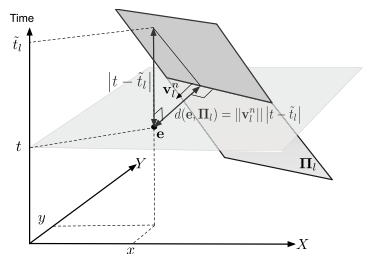
\includegraphics[width = 0.5\linewidth]{distance.png}
    \caption[Distance calculation from event to plane, and plane fitting]{Distance calculation from event to plane, and plane fitting, from \cite{clady2015asynchronous}}
    \label{fig:sec2_plane_distance}
\end{figure}

The way this technique identifies (and tracks corners) is by detecting intersection between these planes, as these intersections correspond to the corner movement through a period of time (Fig.\,\ref{fig:sec2_corner_spacetime}).

\begin{figure}[ht]
    \centering
    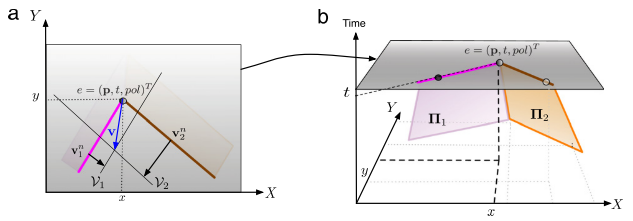
\includegraphics[width = 0.5\linewidth]{corner_spacetime.png}
    \caption[Corner detection using spacetime approach]{Corner are the result of the intersection of lines (edges) at a given timestamp, which themselves result from the spacetime planes that are being estimated, from \cite{clady2015asynchronous}}
    \label{fig:sec2_corner_spacetime}
\end{figure}

\subsubsection{Event-based Harris Corner Detector}
\label{sec:sec2_event_harris}

This technique (from \cite{vasco2016fast}) relies on the Surface of Active Events (SAE), a representation system for events, which keeps track of the timestamp of the most recent event for any given pixel, regardless of polarity, defined by Eq.\,\ref{eq:sec2_sae}. Indeed, it is a spatial representation ($(x,y)$ coordinates, corresponding to each pixel), which can be discretized by assigning a value to each pixel based on its timestamp. Fig.\,\ref{fig:sec2_sae} shows an example of the SAE, where the events are represented from white to grey, as they go from more recent to older.

\printglossaries


\begin{equation}
    \label{eq:sec2_sae}
    SAE:(x,y) \to t
\end{equation}

\begin{figure}[ht]
    \centering
    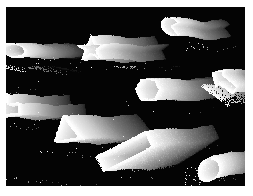
\includegraphics[width = 0.5\linewidth]{sae.png}
    \caption[Representation of the Surface of Active Events (SAE)]{Representation of the Surface of Active Events (SAE), with more recent events being represented in a stronger white, from \cite{mueggler2017fast}}
    \label{fig:sec2_sae}
\end{figure}

Since this discretized representation is now a frame in the classical sense, we can apply the Harris Corner Detector directly to the SAE and identify the corners from these results. 
A more efficient implementation relies on considering only the neighbouring region of an event as it arrives, instead of the whole SAE. As such, only a subset of the SAE is analysed. Since each event, and consequently, each subset, is independent on the other subsets (provided the subsets do not overlap), parallel implementations are possible, and also improve speed.

\subsubsection{SAE-based corner detector}
\label{sec:sec2_sae_corner_detection}


This technique also relies on the SAE representation of events but does not perform any computations. Rather, it performs only comparison operations on a local neighbourhood around the relevant event.

As each event is received, its timestamp is compared with the neighbouring pixels using circular segments (for isotropic response and efficiency), and checked if patterns similar to the one in Fig.\,\ref{fig:sec2_sae_corner} are present (contiguous pixels with decreasing timestamps), as these are typical corner patterns.

Though this method is not as effective, it is much faster, as no computations are performed, and each event can be processed independently (and concurrently in a parallel fashion).

\begin{figure}[ht]
    \centering
    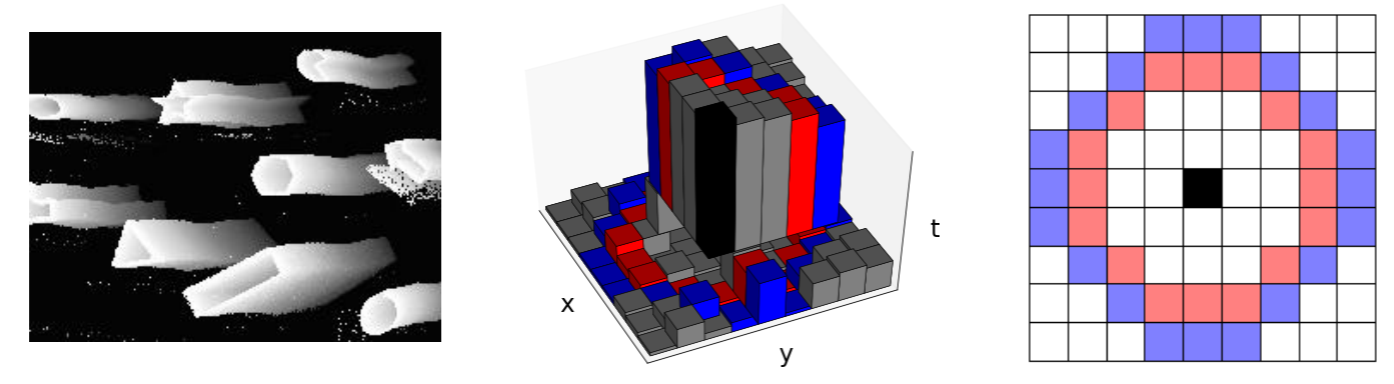
\includegraphics[width = 0.5\linewidth]{sae_corner.png}
    \caption[Corner detection through SAE]{(a) Representation of SAE, on which the comparison filter from (c) is applied, and checked for patterns of decreasing intensity from centre to surrounds, as shown in (b), from \cite{mueggler2017fast}}
    \label{fig:sec2_sae_corner}
\end{figure}

\section{Feature tracking}
\label{sec:sec2_feature_tracking}

ESTA PARTE PRECISA DE TRABALHO, ESTOU UM POUCO INCERTO SE VALE A PENA INCLUIR SIFT E SURF (PELO MENOS DA FORMA COMO ESTÁ)

Having identified features, an important step is being able to match them or track them across multiple frames. As such, it is important to choose features which are unique and not easily mismatched (distinct features), as well as features that are easy to reidentify from multiple angles (robust and stable features, invariant to viewing direction and distance, and illumination variances).

A simple approach is to use a global minimization approach through the Sum of Squared Distances (SSD) between the features being proposed as a match, with the underlying principle that matching features are close to each other in consecutive frames. However, this is not always the case. Also, this approach complicates feature reidentification whenever it exits and re-enters the frame, and is also slow. This technique is better suited for template tracking across frames, assuming rigid body motion, which is not always the case, with independent feature movement.

To facilitate feature matching in classical cameras, along with the features detected (interest points), image descriptors around these points are also preserved, which are then compared for matching. This approach is used by Scale-Invariant Feature Transform (SIFT \cite{lowe1999object}), Speeded Up Robust Features (SURF \cite{bay2006surf}) and similar approaches.

\subsection{SIFT features}
\subsubsection{SIFT detection}
VALE A PENA FALAR DA DETECAO OU SO DOS DESCRITORES????

Features of interest are designated as keypoints in the SIFT framework. This detector uses blobs as keypoints, and relies on the Difference of Gaussians (DoG) to extract keypoints, which are invariant to translation, scaling and rotation.

A pyramid of images of different scales is generated, and for each scale, multiple convolutions with Gaussian kernels are performed (which effectively blurs the images). For each scale, a difference between images (Difference of Gaussians) is performed, and maximum and minimum across scales are kept.

\subsubsection{SIFT descriptors}

Each keypoint has a corresponding descriptor. For each keypoint, a grid of  4x4 blocks is created, each containing 4x4 sub-blocks. For each sub-block, its main orientation is estimated, and all 16 sub-block orientation are condensed into a bin with 8 directions. As such, each feature has a 4x4 blocks x 8 orientation bin which creates a 128D descriptor.

The relevance of the descriptors is when matching, since a variation of the k-d tree algorithm (called the best-bin-first search method) is used to compare and match keypoints fast and correctly across multiple frames.

\subsection{SURF features}
\subsubsection{SURF detection}
VALE A PENA FALAR DA DETECAO OU SO DOS DESCRITORES????

Features of interest detected using the determinant of the Hessian matrix (technique similar to the Harris corner detector), using the same pyramid approach.


\subsubsection{SURF descriptors}

Each keypoint has a corresponding descriptor. For each keypoint, a grid of  4x4 blocks is created, which record orientation using Haar wavelet functions. Each block registers 4 components, resulting in 4x4 grid x 4 components, resulting in a 64D descriptor for each keypoint.

These descriptors are then used for matching features across frames, like with SIFT.

\subsection{Event cameras}

ESTA PARTE JA ME PARECE MAIS ROBUSTA

For event cameras, a typical choice of features, as previously presented, are corners. However, the choice of descriptors for matching and tracking is not yet as developed as for classic cameras.

\subsubsection{SSD}

A first approach to feature matching across frames is to rely on the fast nature of events, and to create pseudo-frames by combining features over a timeslice (accumulation of events for a given interval). The features of both pseudo-frames can then be matched using SSD, assuming a proximity between features in consecutive pseudo-frames. 

Nevertheless, this approach is not ideal, as a critical parameter is the time of integration in the timeslice, which does not take full advantage of the nature of events and event cameras, and could be so slow as to have the same temporal resolution as conventional cameras.

\subsubsection{Spatiotemporal tracking}

The technique presented in Section\,\ref{sec:sec2_space_time} for corner detection is also able to track these corners across multiple timestamps, since the plane and line fitting that are performed in the spatio-temporal representation of events for edges and corners, respectively, implicitly estimates their motion and position across time.

However, since no descriptors or identifiers are being registered, some problems arise when features leave the camera space and are recaptured later, as well as situations where multiple corners overlap and end up merging together. This is particular true for corners from organic features, as opposed to artificial structures.


\subsubsection{EKLT}

EKLT (\cite{gehrig2020eklt}) is a hybrid feature tracking technique that is able to merge information from conventional cameras and events (and hence is more suitable for the new generation of DAVIS event cameras), that tracks corners across time. The method is based on the Lucas-Kanade tracker, hence the name EKLT (event-based Lunas-Kanade tracking).

This method tracks corners, as they are easy to recognize in both conventional cameras (Section\,\ref{sec:sec2_classic_corner_detection}), and correspond to areas with high event generation, that can be detected using event corner detectors as well (Section\,\ref{sec:sec2_sae_corner_detection}).

The idea behind this tracker is to detect features using a conventional frame, which are then tracked using events until a new frame arrives, at which point the estimation from events is compared to the corner detection in the new frame, in essence correcting this estimation. If the feature is not detected, it is still tracked in event space, as subsequent frames may re-detect missed features. This approach is particularly useful in high-speed movements, where motion blur becomes a problem for frames, but not for events.

This comparison between frames and events is crucial, and the key concept is "image variation in a frame patch". As previously discussed (Section\,\ref{sec:sec2_event}), event cameras respond to brightness changes in the environment. Therefore, it is not farfetched to compare events to image gradients, as zones with higher gradients in the world are precisely the ones that produce the most events. In fact, integration (accumulation) of events over a period of time produce results that are very similar to the gradient of the image, as shown in Fig.\,\ref{fig:sec2_gradient_comparison}.

\begin{figure}[ht]
	\centering
		\begin{tabular}{cc}
		   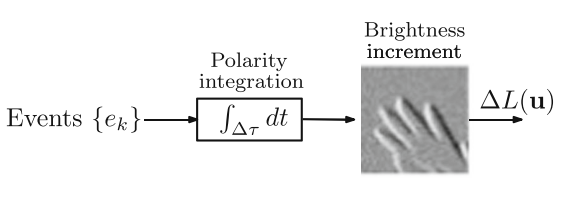
\includegraphics[width=0.45\linewidth]{gradient1.png} &
		   \hspace{1cm} 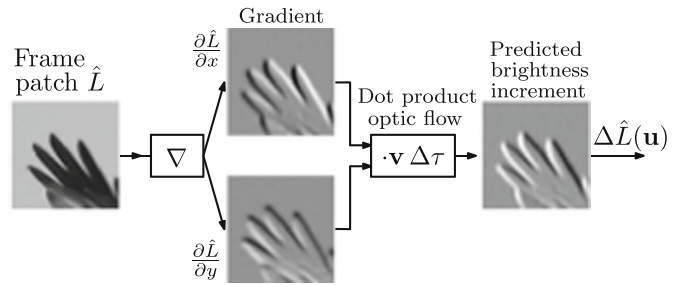
\includegraphics[width=0.45\linewidth]{gradient2.png} \\
		   (a) & (b)  \\
		\end{tabular}
	\caption[Comparison of the brightness change from event integration with the brightness change from image gradient]{Comparison of the brightness change from event integration (a), versus the brightness change from image gradient (b), from \cite{gehrig2020eklt}}
	\label{fig:sec2_gradient_comparison}
\end{figure}

This is the idea at the core of this approach, as the brightness change behaves as the descriptor for the features, and are used as patches for a Lucas-Kanade inspired patch comparison and matching, using both the patch and estimated velocity (estimated through events), using the cost function \eqref{eq:sec2_cost_eklt}, where $\Delta L$ denotes changes from events, $\Delta \hat{L}$ denotes gradients from frames, and $u$ denotes the image, $p$ the warp parameters, and $v$ the velocity. $p$ and $v$ are used as the starting values for the optimizer that minimizes the functional \eqref{eq:sec2_cost_eklt}, and are modified during the optimization process.

\begin{equation}
    \label{eq:sec2_cost_eklt}
    \min_{p,v} \left \| \Delta L(u) - \Delta \hat{L}(u,p,v)) \right \| ^2
\end{equation}

While a new frame is not received, the corner is tracked in event space and the local patch is being created for comparison with a frame patch created from image gradients, as shown in Fig.\,\ref{fig:sec2_eklt_block}.

\begin{figure}[ht]
    \centering
    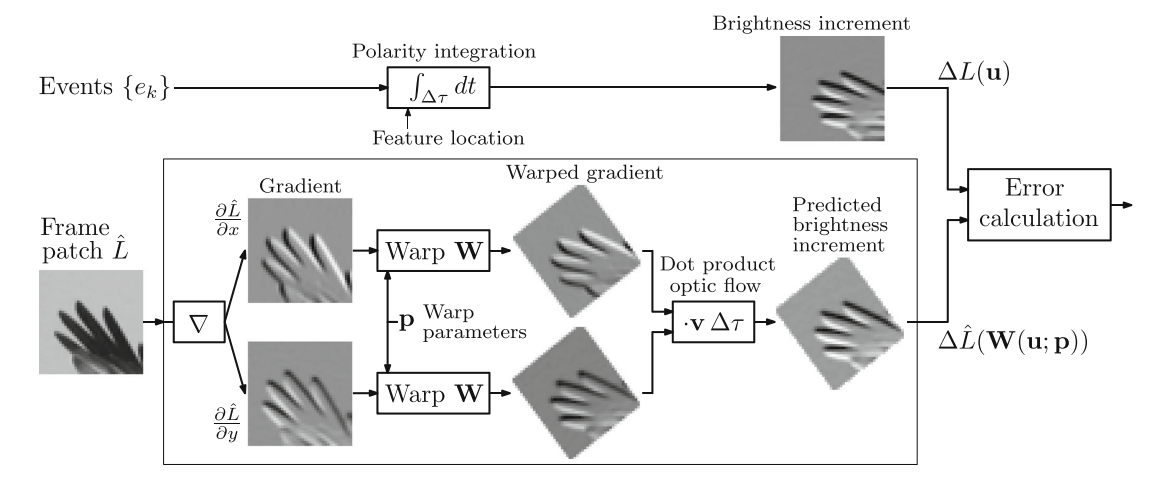
\includegraphics[width = 1\linewidth]{framework.png}
    \caption[Block diagram of EKLT]{Block diagram of EKLT, showing the comparison between brightness changes from images and events, from \cite{gehrig2020eklt}}
    \label{fig:sec2_eklt_block}
\end{figure}

It is worth noting, however, that the dependence on corners may present a problem for low-textured, or highly organic environments, where high quality corners are not always present.
\section{Lie groups and Lie Algebra}
\label{sec:sec2_lie}

INCOMPLETO

\subsection{Algebraic groups}
\label{sec:sec2_groups}

An algebraic group is an algebraic structure with its corresponding operation set. Considering group $A$ and operator $\ast$, the following properties must hold for a structure to be a group.

\begin{itemize}
    \item Closure: $\forall a_1,a_2 \in A, a_1 \ast a_2 \in A$ 
    \item Associativity: $\forall a_1,a_2,a_3 \in A, (a_1 \ast a_2) \ast a_3 = a_1 \ast (a_2 \ast a_3)$
    \item Identity: $\exists a_0 \in A, s.t. \forall a \in A, a_0 \ast a = a \ast a_0 = a$
    \item Inverse: $\forall a \in A, \exists a^{-1} \in A, s.t., a \ast a^{-1} = a_0$
\end{itemize}

A Lie group is an algebraic group that is a smooth differentiable manifold. Furthermore, the operator and the inversion are smooth functions.

\subsection{Lie algebra}
\label{sec:sec2_lie_algebra}

Each Lie group has an associated Lie algebra, corresponding to the tangent space around the identity element of the group, which means that the Lie algebra is a vector space obtained by differentiating the group at the identity transformation. As such, the Lie group representation is desirable when we want to represent differential quantities pertaining to the group, such as velocity and covariance, which are well-represented in the in the tangent space around the transformation, in particular because we can convert any element of the tangent space exactly into a transformation in
the group through the exponential map, and the adjoint transforms tangent vectors from one tangent space to another.

\subsubsection{Exponential and logarithmic maps}

The exponential and logarithmic map allows the transfer of elements between
the Lie group and the corresponding Lie algebra. The exponential map locally maps an element of the tangent space to the group, and  the logarithmic map of a Lie group provides the "inverse operation", transferring elements from the Lie group to its tangent space.
%\section{Unscented Kalman Filter (UKF)}
%\label{sec:sec2_ufk}
\section{Sensor Fusion and Filtering}
\label{sec:sec_filtering}

It is common to have multiple sensors in a system that produce complementary or redundant readings of the world and/or the state of the system. This may be for several reasons, such as sensor noise, sampling rate, and robustness, among others. For example, one sensor may report information on velocity, whereas another reports on position. These two quantities are related through movement equations, and can be considered redundant, but by combining different types of readings, global uncertainties on the system can be reduced, and limitations of the single sensor may be overcome.

However, how to use use and fuse the readings from multiple sensors is itself a critical part. In this work, the event camera was used in conjunction with an IMU, and so fusing the visual information with inertial information was needed. The solution used was an Unscented Kalman Filter (UKF) (explained in Section\,\ref{sec:sec2_ukf}), which is described in Section\,\ref{sec:sec3_ukf}. The UKF is an extension to the Kalman Filter (explained in Section\,\ref{sec:sec2_kf}) applicable to nonlinear systems.

\subsection{Kalman Filter}
\label{sec:sec2_kf}

The Kalman Filter \cite{kalman1960new} is an algorithm that can be applied when we have a linear system that follows the model equations \eqref{eq:sec2_kf_pred} (the system equation) and \eqref{eq:sec2_kf_meas} (the measurement equation), namely a linear system that can be represented with a state $s$ that evolves according to Eq.\,\eqref{eq:sec2_kf_pred} and that can be measured by an observer function \eqref{eq:sec2_kf_meas} that provides $z$, that can be somehow related linearly to the state. $v(k)$ is the state noise process, $u(k)$ is the input to the system, and $w(k)$ is the measurement noise. Both noises are assumed to be zero-mean Gaussian white noise (Eqs.\,\eqref{eq:sec2_noises} and \eqref{eq:sec2_noises_cov}). Furthermore, $x(k) \in \mathbb{R} ^n$, $u(k) \in \mathbb{R} ^m$, $w(k) \in \mathbb{R} ^n$, $v(k) \in \mathbb{R} ^q$, and $y(k) \in \mathbb{R} ^q$.

\begin{equation}
    \label{eq:sec2_kf_pred}
    x(k+1) = F x(k) + B u(k) + G v(k)
\end{equation}
\begin{equation}
    \label{eq:sec2_kf_meas}
    z(k) = H x(k) + w(k)
\end{equation}

\begin{equation}
    \label{eq:sec2_noises}
    E(w(k)) = E(v(k)) = 0
\end{equation}
\begin{equation}
    \label{eq:sec2_noises_cov}
    \begin{bmatrix}
        \bigl(\begin{smallmatrix}
        w(k)\\ 
        v(k)
        \end{smallmatrix}\bigr) &\bigl(\begin{smallmatrix}
        w(m)^T & v(m)^T
        \end{smallmatrix}\bigr) 
        \end{bmatrix}
        =
        \begin{bmatrix}
        R_1 &0 \\ 
         0 & R_2 
        \end{bmatrix}
        \delta(k-m)
\end{equation}

With this formulation, the optimal estimator is given by a set of equations that relate to the prediction of the state based on the input to the system (Eqs.\,\eqref{eq:sec2_kf_pred1} to \eqref{eq:sec2_kf_pred2}), and another set related to the update and correction of the estimate (Eqs.\,\eqref{eq:sec2_kf_obs1} to \eqref{eq:sec2_kf_obs3}), provided by the measurement. 

\begin{equation}
    \label{eq:sec2_kf_pred1}
    \hat{x}(k+1 | k) = F \hat{x}(k | k) + B u(k)
\end{equation}
\begin{equation}
    \label{eq:sec2_kf_pred2}
    P(k+1|k) = F P(k|k) F^T + G R_1 G^T
\end{equation}

\begin{equation}
    \label{eq:sec2_kf_obs1}
     K(k) = P(k|k-1) H^T \left[  H P(k|k-1) H^T + R_2 \right]^{-1}
\end{equation}
\begin{equation}
    \label{eq:sec2_kf_obs2}
    \hat{x}(k | k) = \hat{x}(k | k-1) + K(k) \left [ z(k) - H \hat{x}(k | k-1) \right ]
\end{equation}
\begin{equation}
    \label{eq:sec2_kf_obs3}
    P(k|k) = \left[ I - K(k) H \right] P(k|k-1)
\end{equation}

The Kalman Filter, though optimal, is only applicable to linear systems. As such, alternatives are needed when nonlinear systems are used (which arise particularly in the estimation of rotation in the case of this work). Two extensions to the Kalman Filter are usually considered: the Extended Kalman Filter (EKF) (presented in Section\,\ref{sec:sec2_ekf}) and the Unscented Kalman Filter (UKF) (presented in  Section\,\ref{sec:sec2_ukf}).

\subsection{Extended Kalman Filter (EKF)}
\label{sec:sec2_ekf}

The Extended Kalman Filter (EKF) is an extension to the Kalman Filter when the system or the measurements from the system are nonlinear, such as the one in \eqref{eq:sec2_ekf_system_pred} and \eqref{eq:sec2_ekf_system_obs}, where functions $f$ and/or $h$ are nonlinear functions. In this case, the system cannot be written in matrix notation (such as Eqs.\,\eqref{eq:sec2_kf_pred} and \eqref{eq:sec2_kf_meas}).%, where $x(k)$ is the $n$-dimensional state of the system at timestep k, $u(k)$ is the input vector, $v(k)$ is the q-dimensional state noise process, $z(k)$ is the observation vector and $w(k)$ is the measurement noise. $v(k)$ and $w(k)$ are zero-mean noises. 

\begin{equation}
    \label{eq:sec2_ekf_system_pred}
    x(k+1) = f(x(k),u(k),v(k))
\end{equation}
\begin{equation}
    \label{eq:sec2_ekf_system_obs}
    z(k)=h(x(k), u(k)) + w(k)
\end{equation}

 As such, there are no $F$ or $H$ matrices that can be used for uncertainty propagation (Eqs.\,\eqref{eq:sec2_kf_pred2} and \eqref{eq:sec2_kf_obs3}), since the system is nonlinear, and therefore functions $f$ and/or $h$ cannot be written as a linear combination of the input variables. Furthermore, due to the nonlinear nature of the system, the covariance $P$ would not preserve the Gaussian nature of the noise.

 EKF solves this problem by linearizing the system dynamics around the predicted and filtered estimates of the state, at each cycle, as shown in Eqs.\,\eqref{eq:sec2_ekf_lin_pre} and \eqref{eq:sec2_ekf_lin_meas}, so that a matrix $F_{k+1}$ and $H_{k+1}$ are generated at each cycle, suitable for use in Eqs.\,\eqref{eq:sec2_kf_pred2} and \eqref{eq:sec2_kf_obs3}, as if the system was linear.

 \begin{equation}
    \label{eq:sec2_ekf_lin_pre}
    F_{k+1}=\left. \frac{\partial f}{\partial x}\right|_{\hat{x}_{k+1}|k, u_k}
\end{equation}
\begin{equation}
    \label{eq:sec2_ekf_lin_meas}
    H_{k+1}=\left. \frac{\partial h}{\partial x}\right|_{\hat{x}_{k+1}|k}
\end{equation}

Clearly, this filter is not optimal, as it does not contemplate the full system model, as well as the effect of the noise on the system. Moreover, the need for the linearization of the model can be cumbersome for large systems. 

Nevertheless, the EKF is a simple extension to the Kalman Filter that allows its usage with nonlinear systems, and generally obtains positive results.

\subsection{Unscented Kalman Filter (UKF)}
\label{sec:sec2_ukf}

The Unscented Kalman Filter (UKF) (\cite{julier1997new}) is another extension to the Kalman Filter when the system or the measurements from the system are nonlinear, such as the one in \eqref{eq:sec2_ukf_system_pred} and \eqref{eq:sec2_ukf_system_obs}. This situation is similar to the one in the EKF (Section\,\ref{sec:sec2_ekf})%, where $x(k)$ is the $n$-dimensional state of the system at timestep k, $u(k)$ is the input vector, $v(k)$ is the q-dimensional state noise process, $z(k)$ is the observation vector and $w(k)$ is the measurement noise. $v(k)$ and $w(k)$ are zero-mean noises. 

\begin{equation}
    \label{eq:sec2_ukf_system_pred}
    x(k+1) = f(x(k),u(k),v(k))
\end{equation}
\begin{equation}
    \label{eq:sec2_ukf_system_obs}
    z(k)=h(x(k), u(k)) + w(k)
\end{equation}

Unlike the Extended Kalman Filter (EKF, Section \ref{sec:sec2_ekf}), which can also be used with nonlinear functions, the UKF does not linearize these functions when propagating the uncertainty, and instead tries to approximate distribution of the output to a Gaussian distribution by using an unscented transform. This procedure works by choosing a set of sigma points ($2L+1$ points, corresponding to 2 points around the current estimate for each dimension in the state vector, plus the mean) which are subject to the nonlinear transformation and used to approximate the output distribution. These points are given by Eqs.\,\eqref{eq:sec2_ukf_sigma1} to \eqref{eq:sec2_ukf_sigma3}, with corresponding weights $W_i$ associated to each point, and is illustrated by Fig.\,\ref{fig:sec2_unscent}. Furthermore, $\bar{x}$ represents the mean of state $x$, $P_{xx}$ its covariance, $i \in [1,2n]$, and $\kappa \in \mathbb{R}$ is a tuning parameter.

\begin{equation}
    \label{eq:sec2_ukf_sigma1}
    \chi_0 = \bar{x}, W_0 = k/(n+\kappa)
\end{equation}
\begin{equation}
    \label{eq:sec2_ukf_sigma2}
    \chi_i = \bar{x} + \left( \sqrt{(n+k)P_{xx}} \right), W_i = 1/2(n+\kappa)
\end{equation}
\begin{equation}
    \label{eq:sec2_ukf_sigma3}
    \chi_{i+n} = \bar{x} - \left( \sqrt{(n+k)P_{xx}} \right), W_{i+n} = 1/2(n+\kappa)
\end{equation}

\begin{figure}[ht]
    \centering
    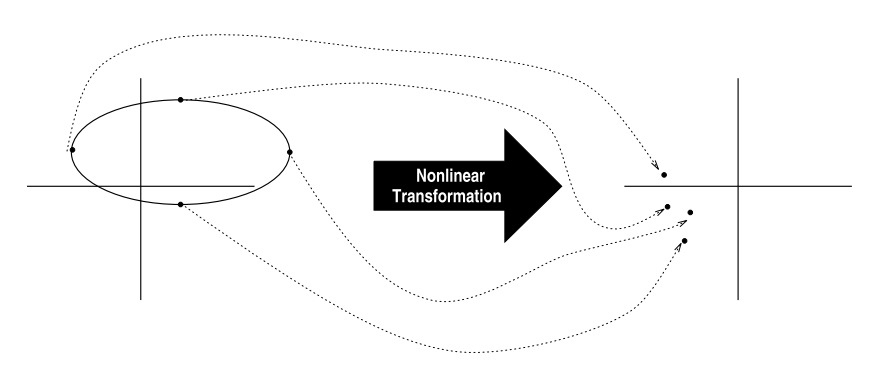
\includegraphics[width = 1\linewidth]{unscent.png}
    \caption[The principle of the Unscented Transform]{The principle of the Unscented Transform, from \cite{julier1997new}}
    \label{fig:sec2_unscent}
\end{figure}

The transformation procedure is then given by Eqs.\,\eqref{eq:sec2_ukf_sigma_exp1} to \eqref{eq:sec2_ukf_sigma_exp3}.

\begin{equation}
    \label{eq:sec2_ukf_sigma_exp1}
    y_i=f(\chi_i)
\end{equation}
\begin{equation}
    \label{eq:sec2_ukf_sigma_exp2}
    \bar{y} = \sum_{i=0}^{2n} W_i y_i
\end{equation}
\begin{equation}
    \label{eq:sec2_ukf_sigma_exp3}
    P_{yy} = \sum_{i=0}^{2n} \left( y_i - \bar{y} \right) \left( y_i - \bar{y} \right) ^T
\end{equation}

This transformation allows us to have the mean and covariance associated with the nonlinear process, without the need to linearize it beforehand, producing a better approximation as well, and these values can then be used in the filter, as shown in Eqs.\,\eqref{eq:sec2_ukf_1} to \eqref{eq:sec2_ukf_7}.

\begin{equation}
    \label{eq:sec2_ukf_1}
    \chi_i (k+1|k) = f (\chi_i(k|k),u(k))
\end{equation}
\begin{equation}
    \label{eq:sec2_ukf_2}
    \hat{x}(k+1|k) = \sum_{i=0}^{2n} W_i  \chi_i (k+1|k) 
\end{equation}
\begin{equation}
    \label{eq:sec2_ukf_3}
    P(k+1|k) = \sum_{i=0}^{2n} W_i \left[  \chi_i (k+1|k) - \hat{x}(k+1|k) \right]  \left[  \chi_i (k+1|k) - \hat{x}(k+1|k) \right]^T
\end{equation}

\begin{equation}
    \label{eq:sec2_ukf_4}
    Z_i(k+1|k) = h(\chi_i (k+1|k), u(k))
\end{equation}
\begin{equation}
    \label{eq:sec2_ukf_5}
    \hat{z}(k+1|k) = \sum_{i=0}^{2n} W_i Z_i(k+1|k)
\end{equation}
\begin{equation}
    \label{eq:sec2_ukf_6}
    P_{vv}(k+1|k) = R_1 + \sum_{i=0}^{2n} W_i \left[ Z_i(k|k-1) - \hat{z}(k+1|k) \right] \left[ Z_i(k|k-1) - \hat{z}(k+1|k) \right]^T
\end{equation}
\begin{equation}
    \label{eq:sec2_ukf_7}
    P_{xz} = \sum_{i=0}^{2n} W_i \left[ \chi_i(k|k-1) - \hat{x}(k+1|k) \right] \left[ Z_i(k|k-1) - \hat{z}(k+1|k) \right]^T
\end{equation}

By using the UKF, it is not needed to linearize the system equations, which results in a better approximation of the uncertainty of the estimate, since the nonlinearities of the system are somewhat taken into account. Furthermore, the use of the unscented transform also makes the filter more robust to noise (\cite{wan2000unscented}).

\subsection{Square-Root Unscented Kalman Filter (Sr-UKF)}
\label{sec:sec2_sr_ukf}


\section{Procrustes approach}
\label{sec2_5:sec_procrutes_approach}

In \cite{mariana2019}, approaches based on the

\chapter{Methods}
\label{sec:sec3}

\epigraph{``Begin at the beginning," the King said gravely, ``and go on till you
come to the end: then stop."}{--- \textup{Lewis Carroll}, Alice in Wonderland}

Intro to section 3
\section{Sensor calibration}
\label{sec:sec3_calibration}

\subsection{Camera}
\label{sec:sec3_cam_calib}

PASSAR A PARTE EXPERIMENTAL DO CAPITULO 2 PARA AQUI.

\subsection{IMU}
\label{sec:sec3_imu_calib}
\section{UKF approach}
\label{sec3:sec_ukf_approach}

The second solution implemented was based on \cite{brossard2017unscented}. It consists of an Unscented Kalman Filter that combines visual and inertial information through an event camera and an IMU. The filter estimates 



\appendix
%\section{Appendix name}


%\section{Appendix name}



\bibliographystyle{apalike}
\bibliography{ref}

\end{document}
